%%%%%%%%%%%%%%%%%%%%%%%%%%%%%%%%%%%%%%%%%%%%%%%%%%%%%%%%%%%%%%%%%%%%%%%%%%
%%
%%	Author Submission Template for Operations Research (OPRE)
%%	INFORMS, <informs@informs.org>
%%	Ver. 1.00, June 2024
%%
%%%%%%%%%%%%%%%%%%%%%%%%%%%%%%%%%%%%%%%%%%%%%%%%%%%%%%%%%%%%%%%%%%%%%%%%%%
%
% Use dblanonrev for Double Anonymous Review submission
% Use sglanonrev for Single Anonymous Review submission
% For example, submission to INFORMS Mathematics of Operation Research, MOOR will have
% \documentclass[moor,dblanonrev]{informs4}
%
% \documentclass[opre,dblanonrev]{informs4}
\documentclass[opre,sglanonrev]{informs4}
\usepackage{eqndefns-left} % For checking the display equation width and equation environment definitions %
\RequirePackage{tgtermes}
\RequirePackage{newtxtext}
\RequirePackage{newtxmath}
\RequirePackage{bm}
\RequirePackage{endnotes}

%\OneAndAHalfSpacedXI
\OneAndAHalfSpacedXII % Current default line spacing
%%\DoubleSpacedXI
%%\DoubleSpacedXII

% Optional LaTeX Packages
\usepackage{algorithm}
\usepackage{algpseudocode}
\usepackage{tikz}
\usepackage{algorithm}
\usepackage{algpseudocode} % 这是关键宏包
\usepackage{amsmath}       % 用于数学公式
\newcommand{\var}[1]{\mathit{#1}} % 自定义命令,用于使变量名显示为斜体
% Private macros here (check that there is no clash with the style)
\usepackage[title]{appendix} % 导入 appendix 包

\usepackage{multirow}
\usepackage{graphicx}
\usepackage{array}
\usepackage{booktabs} % 用于更漂亮的表格线

% Natbib setup for author-number style
\usepackage{natbib}
 \bibpunct[, ]{(}{)}{,}{a}{}{,}%
 \def\bibfont{\small}%
 \def\bibsep{\smallskipamount}%
 \def\bibhang{24pt}%
 \def\newblock{\ }%
 \def\BIBand{and}%


%% Setup of the equation numbering system. Outcomment only one.
%% Preferred default is the first option.
\EquationsNumberedThrough    % Default: (1), (2), ...
%\EquationsNumberedBySection % (1.1), (1.2), ...

%% Setup of theorem styles. Outcomment only one.
%% Preferred default is the first option.
\TheoremsNumberedThrough     % Preferred (Theorem 1, Lemma 1, Theorem 2)
%\TheoremsNumberedByChapter  % (Theorem 1.1, Lema 1.1, Theorem 1.2)
\ECRepeatTheorems  %  

% For new submissions, leave this number blank.
% For revisions, input the manuscript number assigned by the on-line
% system along with a suffix ".Rx" where x is the revision number.
\MANUSCRIPTNO{MOOR-0001-2024.00}

%%%%%%%%%%%%%%%%
\begin{document}
%%%%%%%%%%%%%%%%

\RUNTITLE{Module design for pilots training with full flight simulator}

\TITLE{Module Design for Pilots Training with Full Flight Simulator}



\ABSTRACT{
	This study addresses a practical problem in the design of training modules for pilots with Full Flight Simulators (FFS), using operations research techniques. FFSs are highly precise tools that accurately replicate real-world flight scenarios, making them indispensable for pilot training and evaluation. Given their high cost and limited availability, airlines must strategically design modules for pilots’ periodic recurrent assessments. To enhance aviation safety, we formulate a combinatorial optimization objective function to select a set of modules that minimizes a pilot’s lowest score, enabling early detection of potential weaknesses. Our research underscores the importance of accounting for correlations in pilots’ performance across modules. To this end, we develop a suite of optimization methods and provide corresponding managerial insights. Extensive experimental evaluations demonstrate that our approach significantly outperforms traditional methods reliant on intuition and experience.
}% 
\FUNDING{This research was supported by [grant number, funding agency].}

%Supplemental Material:
%Data Ethics & Reproducibility Note:

% Sample
\KEYWORDS{module design, Full Flight Simulators, simulation optimization}

\maketitle
%%%%%%%%%%%%%%%%%%%%%%%%%%%%%%%%%%%%%%%%%%%%%%%%%%%%%%%%%%%%%%%%%%%%%%

% Text of your paper here

\section{Background}
% Introducing the Full Flight Simulator
The Full Flight Simulator (FFS) is a highly sophisticated flight training device designed to replicate the cockpit environment and operational dynamics of a specific aircraft model with exceptional fidelity \citep{ICAO2015}. 
%Typically mounted on a six-degree-of-freedom hydraulic motion platform, the FFS 
It is capable of simulating the entire spectrum of flight operations, from takeoff and cruise to landing, encompassing both routine procedures and complex scenarios such as engine failures, hydraulic system malfunctions, severe weather conditions, and even rare events like bird strikes or runway contamination \citep{Advancements2024}. The simulation integrates visual, auditory, and tactile feedback, alongside precise instrument readouts and control responses, to provide an immersive experience that closely mirrors actual flight conditions. Certified to the highest standards, such as Level D by aviation authorities like the Federal Aviation Administration (FAA) or the European Union Aviation Safety Agency (EASA), the FFS achieves unparalleled precision, enabling zero flight time training where pilots can qualify without operating an actual aircraft \citep{FAA1995,EASA2020}. However, this extraordinary accuracy comes at a significant cost, with a single FFS unit priced in the tens of millions of dollars, rendering its manufacture and maintenance a substantial financial commitment \citep{CAE7000XR}. Most airlines typically own only a limited number of FFS units outright or instead lease them from manufacturers such as CAE or L3Harris and dedicated flight training centers \citep{IBAAero2023}.

% Explaining the role in pilot training
The primary application of the FFS lies in pilot training and qualification maintenance, with a particular emphasis on mandatory recurrent training to renew licenses. Pursuant to regulations set by the International Civil Aviation Organization (ICAO) and national aviation authorities, pilots are required to undergo recurrent training every six to twelve months, typically conducted in an FFS, to validate their proficiency \citep{Flightradar2024}. During qualification assessments, pilots are evaluated through a series of subjects designed to test their ability to manage diverse operational challenges. These subjects are carefully crafted based on real-world flight data and historical incident analyses %, ensuring relevance to actual flight conditions 
\citep{NTSB2012}. Common subjects include ``Engine Failure on Takeoff,'' where pilots must stabilize the aircraft and execute a safe return to the airport following an engine malfunction immediately after liftoff; ``Low Visibility Approach,'' which tests precision navigation and landing in simulated adverse weather; and ``Emergency Descent and Decompression,'' requiring rapid altitude reduction and oxygen management in response to cabin pressure loss \citep{PilotWorkshops2023}. These assessments, which may span several hours, evaluate technical proficiency, decision-making speed, and crew coordination. Successful completion of these subjects results in license renewal, while deficiencies necessitate further training, ensuring consistent competency across the pilot workforce \citep{EASA2020}.

Given the high cost of FFS and the critical need for regular pilot assessments, airlines must carefully balance budgetary constraints with the demand for efficient and effective evaluations. However, the current practice of selecting assessment subjects is often random or reliant on airlines' experiential judgment, which can fail to identify specific deficiencies or redundantly evaluate areas of established proficiency. This work aims to develop dedicated optimization approaches to enhance the selection of assessment subjects, maximizing the effectiveness of the evaluation process.

Suppose there is a pool of $M$ different training modules from which $m$ are selected in one training session due to cost restriction. Ideally, these $m$ subjects should collectively cover a diverse range of skills to efficiently identify a pilot’s weaknesses. Unlike conventional approaches, our strategy incorporates the correlations and variability in pilot performance across these modules, driven by individual differences in skills such as hand-eye coordination, spatial awareness, and stress resilience. For instance, pilots with strong coordination skills often excel in subjects like ``Precision Approach'' and ``Instrument Flying,'' as both require similar competencies, including accurate interpretation of flight instruments, stable aircraft control, and anticipation of spatial positioning \citep{Damos2003}. As a result, high performance in one module frequently predicts success in the other due to shared skill requirements. Conversely, pilots with superior stress management capabilities may outperform in complex emergency scenarios such as ``Multi-Engine Failure'', but struggle in subjects like ``Crosswind Landing'' if their coordination is less developed \citep{Szczepanska2025}. These correlations arise from overlapping skill sets and selecting multiple highly correlated subjects may lead to redundant testing. %, as pilots who excel or struggle in one are likely to perform similarly in the others. 
Accounting for these correlations is therefore critical in optimizing the selection of assessment modules to enhance training efficiency and safety \citep{Duruaku2024}. 

We illustrate this with a simple example, where we need to select two subjects out of three for a pilot's assessment. From an aviation safety perspective, we aim to select the two subjects that best identify the subject with the lowest score, and thus the assessment metric is the minimum score of the two selected subjects. As an optimization problem, the following objective function is considered:
\begin{equation}
	\min_{x_1, \ x_2} \mathbb{E}[\min\{Y(x_1), \ Y(x_2) \} ], 
	\label{example}
\end{equation}
where $x_1,x_2$ are two selected subjects from the subjects pool $\{A,B,C\}$ and $Y(x_i)$ is the score on $x_i$. The scores of each pilot on these three subjects follow a discrete distribution with three scenarios (shown in Table \ref{tab:example}), each with probability 1/3.
\begin{table}[ht]
	\centering
	\caption{Discrete distribution of the scores}
	\label{tab:example}
	\begin{tabular}{cccc} 
		Scenario & A score & B score & C score \\ \hline 
		1 & 9 & 9.5 & 7.5\\
		2 & 6 & 5 & 8\\
		3 & 10 & 9.5 & 10\\
		Expectation & 8.33 & 8 & 8.5\\
	\end{tabular}
\end{table}
From the table, we can observe that the correlation between scores for subjects A and B is significantly higher than that between A and C or B and C, due to the differing skill requirements for the subjects, as previously discussed. If correlations are ignored, the first two subjects might be chosen (due to their lower mean scores). However, calculations reveal that the latter two subjects should be selected. This is precisely because their lower correlation allows them to more independently yield lower scores, increasing the likelihood of identifying the pilot’s weakest performance. Therefore, we need to design an optimization method that fully accounts for the correlations between scores of different subjects.

%%%%%%%%%%%%%%%%%%%%%%%%%%%%%%%%%%%%%%%%%%%%%%%%%%%%%%%%%%%%%%%%%%%%%%%%%%%%%%%%%%%%%%%%%%%%%%%%%%%%%%%%%%%%%%%%%%%%%%%%%%%%%%%%%%%%%%
%%%%%%%%%%%%%%%%%%%%%%%%%%%%%%%%%%%%%%%%%%%%%%%%%%%%%%%%%%%%%%%%%%%%%%%%%%%%%%%%%%%%%%%%%%%%%%%%%%%%%%%%%%%%%%%%%%%%%%%%%%%%%%%%%%%%%%
%%%%%%%%%%%%%%%%%%%%%%%%%%%%%%%%%%%%%%%%%%%%%%%%%%%%%%%%%%%%%%%%%%%%%%%%%%%%%%%%%%%%%%%%%%%%%%%%%%%%%%%%%%%%%%%%%%%%%%%%%%%%%%%%%%%%%%%%%%%%%%%%%%%%%%%%%%%%%%%%%%%%%%%%%%%%%%%%%%%%%%%%%%%%%%%%%%%%%%%%%%%%%%%%%%%%%%%%%%%%%%%%%%%%%%%%%%%%%%%%%%%%%%%%%%%%%%%%%%%%%%%%%%%%%%%%%%%%%%%%%%%%%%%%%%%%%%%%%%%%%%%%%%%%%%%%%%%%%%%%%%%%%%%%%%%%%%%%%%%%%%%%%%%%%%%%%%%%%%%%%%%%%%%%%%%%%%%%%%%%%%%%%%%%%%%%%%%%%%%%%%%%%%%%%%%%%%%%%%%%%%%%%%%%%%%%%%%%%%%%%%%%%%%%%%%%%%%%%%%%%%%%%%%%%%%%%%%%%%%%%%%%%%%%%%%%%%%%%%%%%%%%%%%%%%%%%%%%%%%%%%%%%%%%%%%%%%%%
Addressing this problem presents multiple challenges. First, in practical applications, the expected performances of pilots on these subjects are likely unknown. While we can infer correlations between scores based on the skill requirements of different subjects, estimating the mean scores of pilots across these subjects is considerably more difficult. Second, even when the parameters of the score distributions are fully known, computing the expected minimum value of several correlated distributions is inherently complex, particularly when selecting an optimal subset of mm modules from a larger set to minimize this value. This combinatorial optimization problem is computationally challenging and generally does not admit an exact solution, necessitating the use of approximation algorithms. Hence, an approach that simultaneously learns from data of previous test results and optimizes the selection process is necessary.

To address the first challenge of estimating score means, we develop a combinatorial multi-armed bandit (CMAB) algorithm based on a Bayesian framework that assigns a prior distribution to the score means and continuously updates it through iterative testing. This learning framework, however, critically relies on an computational oracle to select near-optimal module combinations at each iteration based on current estimates for the score distributions, which directly confronts the second computational challenge. To tackle the computational complexity challenge, we exploit the submodular structure of our objective function. This key property allows us to develop efficient greedy-style algorithms that serve as effective approximation oracles for module selection. By combining these two components—the Bayesian learning framework and the approximation oracles for combinatorial selection—we create an integrated solution that simultaneously learns from evaluation data and optimizes the selection process. 

This paper addresses a problem of significant practical relevance, representing an innovative effort to apply optimization and operations research algorithms to real-world challenges. Previously, the design of pilot training modules has relied heavily on intuition and experience. Beyond its practical significance, the optimization problem explored here also carries substantial theoretical value, presenting multiple challenges as outlined earlier. Moreover, while related to existing research domains, it exhibits notable distinctions. Our work primarily aligns with two categories of optimization studies. The first is simulation-based optimization \citep{Fu2015}, which employs simulation models to support decision-making in real-world systems (FFS is a highly precise simulation tool). Certain simulation optimization studies account for correlations in experimental results when selecting multiple design alternatives \citep{xie2016bayesian}. These correlations primarily arise from the use of common random numbers in computer simulations. However, no prior work in this field has targeted the same objective function as ours, as most focus on evaluating a single design’s performance without an internal minimization operation. The second category is combinatorial multi-armed bandit research \citep{Chen2013}, where some studies select multiple alternatives and use the best as the evaluation metric, akin to our objective function \eqref{example}. Yet, to the best of our knowledge, none have addressed the complex reward structure in \eqref{example} while simultaneously accounting for correlations among alternatives. Although correlations in CMAB settings have been studied in prior works, these typically focus on simpler reward functions that depend only on marginal statistics rather than the full joint distribution of the selected arms. 

The remainder of the paper is organized as follows. Section \ref{related works} reviews the related works. Section\ref{problem formulation} formulates the objective function. Section \ref{BCUCB} presents our Bayesian Combinatorial Upper Confidence Bound (BCUCB) framework and its regret bound. Section \ref{oracle} develops $\alpha$-approximation oracles to tackle the computational challenge within the BCUCB framework. Section 6 reports numerical experiments. Finally, Section 7 concludes the paper.

\section{Related works}
\label{related works}
We review relevant works in three aspects: existing approaches for pilot training modules design, simulation-based optimization, and combinatorial MAB.

\subsection{Simulation-based optimization}
Simulation-based optimization is a powerful approach for decision-making in complex real-world systems. When direct experimentation is impractical due to cost, feasibility, or other constraints, decision-makers can employ simulation models to evaluate various decision alternatives and identify the optimal solution. Decision-making based on FFS, which provides a high-fidelity simulation of an aircraft, can thus be framed as a simulation optimization problem. Our study aligns with existing research in two key aspects. First, the experimental outcomes of different decision alternatives in our problem exhibit correlations. In simulation optimization, such correlations typically arise from the use of common random numbers (CRN), where experiments across different decisions share identical or related random number streams \citep{fu2004optimal,nelson1995using,nakayama2000multiple,kim2005comparison,xie2016bayesian}. The adoption of CRN enhances the ability to discern differences between decision outcomes. However, unlike traditional studies that focus on selecting a single optimal decision, our problem requires identifying a set of decisions and evaluating them based on their minimum performance metric. The second related aspect pertains to sequential optimization, where multiple decisions are evaluated in each iteration. Existing research in this domain primarily leverages parallel computing resources to accelerate the optimization process, yet the objective remains the selection of a single best decision \citep{wu2016parallel,daulton2021parallel}. Although these approaches differ from our objective function, they utilize similar selection criteria, such as the multi-point Expected Improvement (qEI) metric \citep{ginsbourger2008multi}, to determine the set of decisions tested in each parallel experiment. The qEI metric quantifies the expected improvement of the best-performing decision within a set of parallel evaluations relative to previously tested decisions. Notably, \cite{chevalier2013fast} proposed an exact formulation for computing qEI, which necessitates multiple evaluations of the cumulative distribution function of high-dimensional normal distributions. \cite{wang2020parallel} introduced an approximate gradient-based method to optimize qEI, improving computational efficiency. Recently, \cite{men2023simulation} investigated a problem where the goal is to select a single decision, with the performance evaluated as the minimum value of multiple independent outputs associated with that decision. While these studies are relevant to our work, they primarily address optimization in continuous spaces, and and as noted above, their overarching optimization objectives differ from that considered in our research.


\subsection{Combinatorial MAB} 
Our module selection problem naturally fits into the combinatorial multi-armed bandit (CMAB) framework with semi-bandit feedback, where an agent sequentially selects a subset of base arms (super arm) and observes outcomes from all selected arms \citep{pmlr-v28-chen13a}. The CMAB literature predominantly makes two simplifying assumptions: either base arms are \emph{mutually independent} \citep{10.5555/3737916.3740755, Combes2015CombinatorialBR, 10.1145/3410220.3453926}, or the reward function is \emph{linear} in base arm outcomes or depends only on \emph{marginal means} \citep{Demirel2021CombinatorialGP, Kveton2015CombinatorialCB}. In contrast, our problem requires accounting for the full joint distribution's influence on the non-linear minimum-based reward function. Our work is most closely related to \citep{Chen2016CombinatorialMB}, who also consider the expected maximum of selected arms as the reward function but do not incorporate correlations between base arms. \citep{Wang2023CombinatorialBF} also examines a similar maximum reward function but under a more restrictive full-bandit feedback setting with discrete outcomes, whereas we consider continuous distributions with semi-bandit feedback. In an orthogonal direction, \citep{Degenne2016CombinatorialSW} considers correlated base arms with a known covariance matrix under a sub-Gaussian assumption, which aligns with our setting in terms of correlation structure, but focuses on linear reward functions, which fundamentally differ from our minimum-based reward structure that requires complete joint distribution information.

\section{Problem formulation}
\label{problem formulation}
Our goal is to efficiently identify pilots’ deficiencies through rational module design, with these deficiencies measured by their scores during the module evaluation process. Suppose there are $M$ different training modules from which $m$ are selected in one training session due to the time and cost restriction. Then, we select $m$ modules to maximally expose a pilot’s deficiencies, such that the minimum score across these $m$ modules is as low as possible. The optimization problem can be formulated as follows:
\begin{equation}
	\min_{x_1,...,x_m} \mathbb{E}_\xi[\min\{Y(x_1,\xi),...,Y(x_m,\xi) \} ], 
	\label{obj}
\end{equation}
where $x_1,...,x_m$ represent the $m$ modules in the training session, taken from the module set $\mathcal{X} = \{x_1,...,x_M\}$, and $Y(x_1,\xi)$ is the score the pilot obtain in module $x_i$. It is evaluated through simulation at FFS. In this model, we assume the score vector in the population $\{Y(x_1),...,Y(x_M)\}$ follows a multivariate normal distribution. For each specific person, his score is a sample from this distribution. In equation \eqref{obj}, the random vector $\xi$ is used to illustrate the randomness in this multivariate normal distribution. The inner minimization is to find the minimum score one pilot obtain across the given $m$ training modules. We take the minimum value as we need to find the weakness of the pilots considering flight safety. The outer minimization is the find the best set of training sessions in detecting the pilot inadequacy.

\section{A Combinatorial MAB Algorithm for Unknown Score Means}
\label{BCUCB}
\subsection{Model Formulation}
We assume that the score has Gaussian noise: $Y(x) = Z(x) + \mathcal{N}(0,\sigma(x))$ and the joint distribution for $Y(x)_{x\in\{\mathcal{X}\}}$ is a multivariate normal distribution with mean vector $\theta = [Z(x_1),...,Z(x_M)]^T$ and covariance matrix $\Lambda$. We use a Bayesian approach to model $\theta$ and assume a normal prior:
$$\theta \sim \mathcal{N}(\mu_0, \Sigma_0). $$
As with \cite{xie2016bayesian}, we assume $\Lambda, \mu_0, \Sigma_0$ are known.

The $i$th entry of a vector $v$ is denoted as $v(i)$ and the $(i,j)$th entry of a matrix $M$ is denoted as $M(i,j)$. For an ordered collection of $m$ alternatives ${\bf x}=(x_1,...,x_m)$ with element $x_i \in \{1,...,M\}$ for each $i$, we use $v(\bf x)$ to denote the subvector of $v$ with the $i$th entry equal to $v(x_i)$. We further denote by $M(\bf x, x')$ the $m$-by-$m$ submatrix of $M$ with the $(i,j)$th entry equal to $M(x_i, x_j')$.  

We consider a situation where in each iteration $t$, one pilot will attend $m$ different modules ${\bf x}_t = (x_{t,1},...,x_{t,m})^T$ and we obtain his score vector ${\bf y}_t = (Y(x_{t,1}),...,Y(x_{t,m}))^T$. The conditional distribution of ${\bf y}_t$ is:
$${\bf y}_t | \theta,{\bf x}_t \sim \mathcal{N}(\theta({\bf x}_t), \Lambda({\bf x}_t,{\bf x}_t)). $$ 
Let $\mathbb{X}_t = ({\bf x}_1^T,...,{\bf x}_t^T )$ denote the concatenation of the design points of the previous $t$ iteration and similarly $\mathbb{Y}_t =({\bf y}_1^T,...,{\bf y}_t^T )^T$. Then, the posterior distribution for $\theta$ is:
$$\theta_n|\mathbb{X}_t,\mathbb{Y}_t  \sim \mathcal{N}(\mu_t, \Sigma_t),$$
where for any vector ${\bf x} = (x_1, x_2,...,x_m)$,
$$
	\mu_t({\bf x}) = \mu_0({\bf x}) + \Sigma_0(\bf x, \mathbb{X}_t)(\Sigma_0(\mathbb{X}_n,\mathbb{X}_t) + \Gamma_t)^{-1}(\mathbb{Y}_t-\mu_0(\mathbb{X}_t)),
$$
$$
	\Sigma_n({\bf x},{\bf x}) = \Sigma_0({\bf x},{\bf x}) - \Sigma_0(\bf x, \mathbb{X}_t)(\Sigma_0(\mathbb{X}_t,\mathbb{X}_t) + \Gamma_t)^{-1}\Sigma_0(\mathbb{X}_t, \bf x),
$$
where $\Gamma_t$ can be calculated from the observed samples since we know the covariance matrix $\Lambda$.

\subsection{The BCUCB Algorithm} 
To address the challenge of unknown score means, we propose a Bayesian Combinatorial Upper Confidence Bound (BCUCB) algorithm. This algorithm iteratively maintains a bayesian posterior distribution over the mean scores $\boldsymbol{\theta}$ and leverages an $\alpha$-approximation oracle for module selection.

The algorithm operates in two phases: an initial exploration phase that ensures each module is evaluated at least once, followed by the main optimization phase. At each iteration $t$, the algorithm constructs a lower confidence bound (LCB) estimate $\boldsymbol{\tilde{\mu}}_t = \boldsymbol{\mu}_{t-1} - \boldsymbol{\beta}_t \circ \boldsymbol{\sigma}_{t-1}$ based on the current posterior distribution. This LCB vector is then passed to an $\alpha$-approximation oracle $\mathcal{O}$ that selects a module set $S_t$ aiming to minimize the expected minimum score. The specific design and implementation of this oracle will be detailed in the next section. After evaluating the selected modules on a new pilot, the posterior distribution is updated with the observed scores. The complete procedure is summarized in Algorithm \ref{alg:bcucb_algorithm}.

\begin{algorithm}
\caption{Bayesian Combinatorial Upper Confidence Bound (BCUCB)}
\label{alg:bcucb_algorithm}
\begin{algorithmic}[1]
\Require{Module set $\mathcal{X}$; Covariance matrix $\boldsymbol{\Lambda}$; Prior parameters $\boldsymbol{\mu}_0$, $\boldsymbol{\Sigma}_0$; Oracle $\mathcal{O}$; Iterations $N_0,N$}
\State Initialize $\boldsymbol{\mu}_0$, $\boldsymbol{\Sigma}_0$ and count vector $\mathbf{T}_0 \gets \mathbf{0}$ 
\For{$i = 1$ to $N_0$} \Comment{Initial exploration phase}
	\State Play a super arm $S_i$ that contains module $i$
	\State Observe $\mathbf{y}_i$,Update $(\boldsymbol{\mu}, \boldsymbol{\Sigma},\mathbf{T}_i)$,Calculate $R(S_i)$ \Comment Same as steps 11, 12, and 13
\EndFor
\For{$t = N_0+1$ to $N$} \Comment{Main optimization phase}
    \State $\boldsymbol{\sigma}_{t-1} \gets \sqrt{\text{diag}(\boldsymbol{\Sigma}_{t-1})}$ \Comment{Compute posterior standard deviations}
    \State $\boldsymbol{\beta}_t[x] \gets \sqrt{6 \ln t / \mathbf{T}_{t-1}[x]}$ for each $x \in \mathcal{X}$ \Comment $\mathbf{T}_{t-1}[x]$ represents the number of times module $x$ was observed before round $t-1$
    \State $\boldsymbol{\tilde{\mu}}_t \gets \boldsymbol{\mu}_{t-1} - \boldsymbol{\beta}_t \circ \boldsymbol{\sigma}_{t-1}$ \Comment{Construct LCB-based mean estimate}
    \State $S_t \gets \mathcal{O}(\boldsymbol{\tilde{\mu}}, \boldsymbol{\Lambda})$ \Comment{Query $\alpha$-approximation oracle}
    \State Observe score vector $\mathbf{y}_t$ for modules $S_t$ on a new pilot.
    \State Update $(\boldsymbol{\mu}_t, \boldsymbol{\Sigma}_t)$ with $(\mathbf{y}_t, S_t)$; Update $\mathbf{T}_t[x] \gets \mathbf{T}_t[x] + 1$ for each $x \in S_t$
    \State Calculate $R(S_t) = \mathbb{E}[\min\,\{Y(x) : x \in S_t\}]$, track minimal $R(S_t)$ and corresponding $S_t$ 
\EndFor
\State \Return $S^*$ with minimal $R(S^*)$
\end{algorithmic}
\end{algorithm}

\subsection{Regret analysis}
In this section we bound the regret of Algorithm \ref{alg:bcucb_algorithm}.
First, we derive a concentration inequality that characterizes the uncertainty reduction through Bayesian inference. Let $T_{i,t-1}$ be the number of times module $i$ has been observed before round $t$.
\begin{lemma}
\label{lemma:concentration}
For any module $i \in \mathcal{X}$, any number of observations $n = T_{i,t-1} \geq 1$, and any $\epsilon > 0$, the deviation of the posterior mean $\mu_{t-1}(i)$ from the true mean $\mu(i)$ is bounded by:
$$
\mathrm{Pr}\left[|\mu_{t-1}(i) - \mu(i)| \geq \epsilon \right] \leq \exp\left(-\frac{n \epsilon^2}{2\sigma^2(i)}\right),
$$
where $\sigma^2(i)$ is the noise variance for module $i$.
\end{lemma}

Second, we show two critical properties of our reward $R(S) = \mathbb{E}[\min\,\{Y(x) : x \in S\}]$ that are fundamental to our analysis. Consider two multivariate normal distributions $\mathcal{N}_1$ and $\mathcal{N}_2$ that share the same covariance matrix but have different mean vectors $\boldsymbol{\mu}_1$ and $\boldsymbol{\mu}_2$. We have the following two lemmas:

\begin{lemma}
\label{lemma:monotonicity}
If $\boldsymbol{\mu}_1 \geq \boldsymbol{\mu}_2$ component-wise, then for any super arm $S$, the reward satisfies:
$$
R_{\mathcal{N}_1}(S) \geq R_{\mathcal{N}_2}(S).
$$
\end{lemma}

\begin{lemma}
\label{lemma:lipschitz}
If $|\mu_1(i) - \mu_2(i)| \leq \gamma_i$ for all modules $i \in \mathcal{X}$, then for any super arm $S$, the difference in rewards is bounded by:
$$
|R_{\mathcal{N}_1}(S) - R_{\mathcal{N}_2}(S)| \leq \max_{i \in S} \gamma_i.
$$
\end{lemma}
The lemmas characterize fundamental properties of the reward function. Lemma \ref{lemma:monotonicity} demonstrates its monotonicity with respect to the component-wise ordering of the mean vectors. Lemma \ref{lemma:lipschitz} establishes a bounded difference property, showing that the change in reward is constrained by the maximum change in any constituent module's mean.

Next we define two pivotal events for rounds \(m+1 \leq t \leq T\):
$$
\varepsilon_t = \left\{\exists\, i \in [m] \text{ such that } \left|\hat{\mu}_{T_{i,t-1}}^i - \mu^i\right| \geq \sigma(i)\sqrt{\frac{6\ln t}{T_{i,t-1}}} \right\}
$$
$$
\mathcal{H}_t = \left\{0 < \Delta_{S_t} \leq 2 \max_{i \in S_t} \sigma(i)\sqrt{\frac{6\ln t}{T_{i,t-1}}} \right\}
$$

Then we can get the following lemma:

\begin{lemma}
\label{lemma:decomposition}
The \(\alpha\)-approximation regret over \(T\) rounds satisfies:
$$
\text{Reg}_{P,\alpha}(T) \leq \mathbb{E}\left[\sum_{t=m+1}^{T} \mathbb{I}\{\mathcal{H}_t\} \Delta_{S_t}\right] + \left(\frac{\pi^2}{6} + 1\right) \alpha M m.
$$
\end{lemma}

This result is derived from a regret decomposition based on the event \(\varepsilon_t\):
$
\text{Reg}_{P,\alpha}(T) \leq \mathbb{E}\left[\sum_{t=1}^{m} \Delta_{S_t}\right] + \mathbb{E}\left[\sum_{t=m+1}^{T} \mathbb{I}\{\varepsilon_t\} \Delta_{S_t}\right] + \mathbb{E}\left[\sum_{t=m+1}^{T} \mathbb{I}\{\neg \varepsilon_t\} \Delta_{S_t}\right]
$. The first term corresponds to the initialization phase and can be trivially bounded. The second term is controlled using the concentration inequality from Lemma 1. For the third term, we can employ the properties established in Lemmas 2 and 3 to show that:
$
\mathbb{E}\left[\sum_{t=m+1}^{T} \mathbb{I}\{\neg \varepsilon_t\} \Delta_{S_t}\right] \leq \mathbb{E}\left[\sum_{t=m+1}^{T} \mathbb{I}\{\mathcal{H}_t\} \Delta_{S_t}\right].
$ 

Now, the remaining task reduces to bounding the key quantity \(\mathbb{E}\left[\sum_{t=m+1}^{T} \mathbb{I}\{\mathcal{H}_t\} \Delta_{S_t}\right]\). To bound this term, we proceed with the following strategy. We first demonstrate that whenever event \(\mathcal{H}_t\) occurs, at least one event from a specific collection of events must happen. We then establish an upper bound on the expected number of occurrences for each event in this collection. By combining these individual bounds, we ultimately derive an upper bound for the target term. Finally, we can get the following result:

\begin{theorem}
\label{thm:regret_bound}
The $\alpha$-approximation regret of Algorithm \ref{alg:bcucb_algorithm} over $T$ rounds satisfies the following upper bounds:
\begin{enumerate}
    \item \textbf{Distribution-dependent bound:}
    $$
    \sigma^2 m \sum_{i \in E_B} \frac{2136}{\Delta_{i,\min}} \ln T + \left(\frac{\pi^2}{6} + 1\right) \alpha y_{\text{max}} M.
    $$
    
    \item \textbf{Distribution-independent bound:}
    $$
    93\sigma \sqrt{M m T \ln T} + \left(\frac{\pi^2}{6} + 1\right) \alpha y_{\text{max}} M.
    $$
\end{enumerate}
\end{theorem}


\section{Design of $\alpha$-Approximation Oracles}
\label{oracle}

This section details the design of the $\alpha$-approximation oracle $\mathcal{O}$ used in the BCUCB algorithm given current parameter estimates. That is, we aim to select a limited number of dimensions from a completely known multivariate normal distribution such that the expected value of the minimum score across these dimensions is minimized. It should be noted that, in general, this objective function cannot be simplified into a more computationally convenient form. Existing studies provide closed-form solutions for the expected minimum of two normal distributions \citep{nadarajah2008exact}. However, for more than two normal distributions, prior research remains limited. \cite{clark1961greatest} relied on numerical approximation, that recursively applies a three-variate formula, to compute the expected value of their minimum and has analyzed the accuracy of these approximations through numerical validation. Such computational methods are time-consuming, particularly in our optimization scenario, where we need to repeatedly select $m$ modules and compute the expected value of their minimum scores. Therefore, we aim to derive managerial insights from simple, analytically tractable examples and leverage these insights to develop efficient heuristic methods. This section is divided into two parts: in Section \ref{insights}, we use two simplified examples to obtain some insights; in Section \ref{submodular}, we demonstrate that the objective function is submodular, enabling the use of a greedy algorithm to achieve an efficient and theoretically guaranteed approximation; in Section \ref{heuristic}, we utilize these insights to develop an efficient heuristic method based on greedy approach.

\subsection{Insights from two simple examples}
\label{insights}
This subsection examines two simplified examples to investigate how parameters in a multivariate normal distribution—specifically the mean, correlation, and variance—affect the expected minimum value. The examples include a bivariate normal distribution (Section \ref{bivariate normal}) and a multi-variate scenario with same means, variances, and correlations (Section \ref{multi-variate}). Despite their simplicity, the conclusions and insights from these examples align with intuition and are corroborated by subsequent numerical experiments.

\subsubsection{Bivariate normal example}
\label{bivariate normal}

%We need to compare Eξ1,ξ2[min\text{E}_{\xi_1, \xi_2}[\min \{\mu_1+A\xi_1, \mu_2+B_1\xi_1+B_2\xi_2 \}] and \text{E}_{\xi_1, \xi_2}[\min \{\mu_1+A\xi_1, \mu_2+B\xi_2 \}]\text{E}_{\xi_1, \xi_2}[\min \{\mu_1+A\xi_1, \mu_2+B\xi_2 \}], where \xi_1, \xi_2\xi_1, \xi_2 are independent standard normal random variable. All the coefficients are positive and that B_1^2+B_2^2=B^2B_1^2+B_2^2=B^2.

For any two Gaussian random number $X_1\sim N(\mu_1,\sigma^2_1)$, $X_2\sim N(\mu_2,\sigma^2_2)$ with correlation $\rho$, the expectation $\text{E}[\min\{X_1, X_2\}]$ takes the following form \citep{clark1961greatest}:
$$
\text{E}[\min\{X_1, X_2\}] = \mu_1\Phi(\frac{\mu_2-\mu_1}{\theta}) + \mu_2\Phi(\frac{\mu_1-\mu_2}{\theta}) - \theta \phi(\frac{\mu_2-\mu_1}{\theta} ),
$$
where $\phi$, $\Phi$ are cdf and pdf for standard normal distribution, respectively, and $\theta = \sqrt{\sigma^2_1+\sigma^2_2-2\rho \sigma_1\sigma_2} = \sqrt{\text{var}(X_1-X_2)}$.

Denote $f=\text{E}[\min\{X_1, X_2\}] $. We have:
\begin{equation}
	\frac{\partial f}{\partial \theta} = -\phi(\frac{\mu_2-\mu_1}{\theta})<0,
\end{equation}
\begin{equation}
	\label{rho}
	\frac{\partial f}{\partial \rho} = \frac{\partial f}{\partial \theta} \frac{\partial \theta}{\partial \rho} =  \frac{\sigma_1\sigma_2}{\theta}\phi(\frac{\mu_2-\mu_1}{\theta})>0,
\end{equation}
\begin{equation}
	\label{sigma}
	\frac{\partial f}{\partial \sigma_1} = \frac{\partial f}{\partial \theta} \frac{\partial \theta}{\partial \sigma_1} = -\frac{\sigma_1-\rho\sigma_2}{\theta} \phi(\frac{\mu_2-\mu_1}{\theta}),
\end{equation}
\begin{equation}
	\label{mu}
	\frac{\partial f}{\partial \mu_1} = \Phi( \frac{\mu_2-\mu_1}{\theta})>0.
\end{equation}

We summarize the conclusions is the following lemma:
\begin{lemma}
	In the bivariate normal example, the expectation of the minimum value is smaller when the two variables have smaller expectations and correlations.
\end{lemma}

The relation between $f$ and the variance for each individual variable is not monotone. We can, however, derive some special cases:
	\begin{enumerate}
		\item When $\rho<\frac{\sigma_1}{\sigma_2}$ (specifically when $\rho<0$), a larger value of $\sigma_1$ is preferred.
		\item When $\rho>\frac{\sigma_1}{\sigma_2}$, smaller value of $\sigma_1$ is preferred. This result may appear counter-intuitive. To gain insight, consider a special case where $\rho = 1$ and $\sigma_1<\sigma_2$. In this scenario, $X_1$ and $X_2$ are positively linear dependent, with $ X_1 = \frac{\sigma_1}{\sigma_2} X_2$. Consequently, $X_1$ and $X_2$ always share the same sign. When $X_1, X_2 > 0$, the minimum is $\min\{X_1, X_2\} = X_1 > 0$, which increases with $\sigma_1$. When $X_1, X_2 < 0$, the minimum is $\min\{X_1, X_2\} = X_2 < 0$, which is independent of $\sigma_1$. Thus, a larger $\sigma_1$ increases the objective function value in this case. Although a larger $\sigma_1$ reduces $X_1$ when negative, these negative values do not contribute to the objective function as long as $\sigma_1 < \sigma_2$. This effect diminishes slightly as $\rho$ deviates from 1, but negative values of $X_1$ remain less likely to influence the objective function until $\rho < \frac{\sigma_1}{\sigma_2}$.
	\end{enumerate}


\subsubsection{Multi-variate normal example}
\label{multi-variate}

We consider the following scenario: $m$ normal random numbers $X_1,...,X_m$ with equal mean $\mu$ and equal variance $\sigma^2$. The correlation between each pair of variables is $\rho\geq 0$. We would like to explore the relationship between the objective function  $f = \text{E}[\min\{X_1,...,X_m\}]$ and $\rho$, $\mu$, and $\sigma$.

In this case, each random variable can be represented as $X_i = \mu + \sigma(\sqrt{\rho}W + \sqrt{1-\rho} N_i )$, where $W$ and $N_1,...,N_m$ are i.i.d. standard normal random variables. Then,
$$f = \text{E}[\min\{X_1,...,X_m\}] =  \text{E}[\min\{\mu + \sigma(\sqrt{\rho}W + \sqrt{1-\rho} N_1 ),...,\mu + \sigma(\sqrt{\rho}W + \sqrt{1-\rho} N_m )\}] $$
$$=\mu+ \sigma\text{E}[\min\{\sqrt{\rho}W + \sqrt{1-\rho} N_1 ,...,\sqrt{\rho}W + \sqrt{1-\rho} N_m \}]  $$
$$=\mu + \sigma\text{E}[\sqrt{\rho}W+ \sqrt{1-\rho} \min\{N_1,...,N_m\} ] =\mu + \sigma\sqrt{1-\rho} \text{E}[\min\{N_1,...,N_m\} ]. $$
%This had no analytical solution. Some special cases:
%\begin{enumerate}
%	\item When \rho =1\rho =1, f=\muf=\mu.
%	\item When \rho =0\rho =0, f = \mu+ \sigma\text{E}[\min\{N_1 ,...,N_m \}]f = \mu+ \sigma\text{E}[\min\{N_1 ,...,N_m \}]. 
%\end{enumerate}
Noted that $\text{E}[\min\{N_1 ,...,N_m \}]$ is a constant for a given $m$. It is negative and can be approximated as 
$$-\sqrt{2 \ln m} + \frac{\ln \ln m + \ln 4\pi}{ 2 \sqrt{2 \ln m}}. $$
Hence, $f\approx \mu - \sigma\sqrt{1-\rho}\sqrt{2 \ln m}$. 

We summarize the insights from this example in the following lemma.

\begin{lemma}
	In the simple multi-variate normal example, the expectation of the minimum value is smaller with smaller $\mu$, larger $\sigma$ or smaller $\rho$.
\end{lemma}

For a general multi-variate normal distribution, analyzing the impact of the covariance matrix on the objective function $   f   $ using simple algebra is challenging. However, we can derive the following lemma regarding the influence of the means.
\begin{lemma}
\label{lemma_mean}
	In a general multi-variate normal distribution, if the covariance matrix is fixed, the value of $f$ reduces if the mean vector gets smaller pointwisely.
\end{lemma}

We summarize the managerial insights derived from these examples for decision-making as follows. To achieve a smaller value for the objective function, we should generally select: 
\begin{enumerate}
	\item $m$ Gaussian variables with smaller means;
	\item variables with lower correlations;
	\item variables with larger variances.
\end{enumerate}
According to Lemma \ref{lemma_mean}, when other factors remain constant, a smaller mean vector directly reduces the expected minimum value. Furthermore, regarding the other two points, the lower the correlations and the larger the variances of the $m$ variables, the more independently each variable can take potentially smaller values, thereby reducing the minimum value.




\subsection{Submodularity and Greedy Approximation}
\label{submodular}
We first recall the definition of submodularity. For a finite set $\mathcal{V}$ (the set of all training modules $\mathcal{X}$ in our context), a set function $F: 2^{\mathcal{V}} \to \mathbb{R}$ is \textbf{submodular} if it satisfies the diminishing returns property: for any subsets $S \subseteq T \subseteq \mathcal{V}$ and any element $x \in \mathcal{V} \setminus T$,
$$
F(S \cup \{x\}) - F(S) \geq F(T \cup \{x\}) - F(T).
$$
This means the marginal gain of adding a new element $x$ to a set $S$ is at least as large as the marginal gain of adding the same element to a superset $T$ of $S$.

In our problem, we define the set function for a module subset $S \subseteq \mathcal{X}$ as $R(S) = \mathbb{E}[\min\{Y(x) : x \in S\}]$. Our goal is to minimize $R(S)$. To frame this for a greedy algorithm that maximizes a utility, we define a utility function $U(S) = y_{\text{max}}-R(S)$. Here $y_{\text{max}}$ is the maximum score a pilot could achieve on any module. Then we give the following theorem:

\begin{theorem}
\label{thm:submodular}
Given that the module score vector $\mathbf{Y} = (Y(x_1,\xi),...,Y(x_m,\xi))$ follows a multivariate normal distribution $\mathcal{N}(\boldsymbol{\mu}, \boldsymbol{\Sigma})$. For $S \subseteq \mathcal{X}$, the set function $U(S) = y_{\text{max}}-R(S) = y_{\text{max}}-\mathbb{E}[\min\{Y(x) : x \in S\}]$ is:
\begin{enumerate}
    \item \textbf{Monotone Increasing}: For any $S \subseteq T \subseteq \mathcal{X}$, $U(S) \leq U(T)$.
    \item \textbf{Submodular}: For any $S \subseteq T \subseteq \mathcal{X}$ and any module $x \in \mathcal{X} \setminus T$, $U(S \cup \{x\}) - U(S) \geq U(T \cup \{x\}) - U(T)$.
\end{enumerate}
\end{theorem}

Theorem \ref{thm:submodular} establishes that $U(S)$ is a monotone increasing, submodular function. Therefore, the problem of selecting a set $S$ of size $m$ to maximize $U(S)$ is an instance of maximizing a monotone submodular function under a cardinality constraint.

For this class of problems, the classical greedy algorithm provides a strong approximation guarantee. The algorithm starts with an empty set $S_0 = \emptyset$. At each step $k = 1, ..., m$, it adds the module $x$ that provides the highest marginal gain:
\begin{equation}
x_{k} = \argmax_{x \in \mathcal{X} \setminus S_{k-1}} \left[ U(S_{k-1} \cup \{x\}) - U(S_{k-1}) \right],
\end{equation}
and then updates $S_k = S_{k-1} \cup \{x_k\}$.

\begin{theorem}[\cite{nemhauser1978analysis}]
\label{thm:greedy_guarantee}
Let $S^*$ be the optimal set of size $m$ that maximizes $U(S)$, and let $S^{\text{greedy}}_m$ be the set of size $m$ obtained by the greedy algorithm. If $U$ is a monotone, non-negative, submodular function, then the greedy algorithm achieves the following performance guarantee:
$$
U(S^{\text{greedy}}_m) \geq \left(1 - \frac{1}{e}\right) U(S^*) \approx 0.632 \cdot U(S^*).
$$
\end{theorem}


This theoretical guarantee allows us to use the greedy algorithm as an $\alpha$-approximation oracle with $\alpha = (1 - 1/e)$. However, a direct implementation requires computing the expected minimum value, which remains computationally challenging. While Sample Average Approximation (SAA) can be employed, it requires extensive Monte Carlo simulations and becomes prohibitive for large-scale problems.

\subsection{Efficient Heuristic Oracles}
\label{heuristic}
To address the computational challenge, we derive inspiration from the analytical solution for the bivariate case:

\begin{lemma}[\cite{clark1961greatest}]
\label{lem:bivariate}
For two Gaussian random variables $X_1\sim N(\mu_1,\sigma^2_1)$, $X_2\sim N(\mu_2,\sigma^2_2)$ with correlation $\rho$, the expectation $\mathbb{E}[\min\{X_1, X_2\}]$ has closed-form solution:
$$
\mathbb{E}[\min\{X_1, X_2\}] = \mu_1\Phi(\frac{\mu_2-\mu_1}{\theta}) + \mu_2\Phi(\frac{\mu_1-\mu_2}{\theta}) - \theta \phi(\frac{\mu_2-\mu_1}{\theta} )
$$
where $\theta = \sqrt{\sigma^2_1+\sigma^2_2-2\rho \sigma_1\sigma_2}$, and $\phi$, $\Phi$ are PDF and CDF of standard normal distribution.
\end{lemma}

This analytical insight motivates the development of more efficient heuristic oracles that approximate the marginal gain without expensive numerical integration.

\subsubsection{Improvement-based Oracle}

As established in Section 4.1.1, the expected value of the minimum of two module scores, $\mathbb{E}[\min\{Y(x_1), Y(x_2)\}]$, admits an exact closed-form solution under the bivariate normal distribution assumption. Leveraging this analytical tractability, we define a pairwise measure of deficiency enhancement for any two modules $x_1$ and $x_2$. Specifically, the \textbf{improvement} (Ipr) of incorporating module $x_2$ given a baseline module $x_1$ is defined as:
$$
\text{Ipr}(x_2 | x_1) = \mathbb{E}[\min\{Y(x_1), Y(x_2)\}] - \mathbb{E}[Y(x_1)].
$$
This quantity captures the expected reduction in the minimum score by adding $x_2$ to an assessment already containing $x_1$. It follows directly from the definition that $\text{Ipr}(x_2 | x_1) = 0$ when $x_1$ and $x_2$ are identical.

Next, consider an existing set of selected modules $S = \{x_2, x_3, x_4\}$. We can extend the pairwise improvement concept by defining the marginal improvement of adding a new module $x_1$ to the set $S$ as:
$$
\text{Ipr}(x_1 | S) = \mathbb{E}\left[\min\,\{Y(x) : x \in S \cup \{x_1\}\}\right] - \mathbb{E}\left[\min\,\{Y(x) : x \in S\}\right].
$$
This metric quantifies the expected reduction in the overall minimum score resulting from the inclusion of $x_1$ into the current assessment portfolio $S$.

Now let's consider an extreme case, assuming $x_1$ and $x_2$ are exactly the same (i.e. $\text{Ipr}(x_1|x_2)=0$), regardless of the value of $\text{Ipr}(x_1|x_3)$ and $\text{Ipr}(x_1|x_4)$, the value of $\text{Ipr}(x_1|S)$ is always $0$. This inspires us to speculate that the value of the improvement of module $x_1$ over set $S$ is dominated by pairwise minima: $\underset{x\in S}{{\min}}~\text{Ipr}(x_1|x)$. So we can define the contribution of module $x_1$ to set $S$: 
$$
\text{Ctr}(x_1|S) = \underset{x\in S}{{\min}}~\text{Ipr}(x_1|x)
$$
Here, the contribution measure $\text{Ctr}(x_1|S)$ represents quantifies the reduction potential in the minimum score when adding module $x$ to set $S$.

Based on this we can get our improvement-based approach as follows:

\begin{algorithm}
\caption{Improvement-based Oracle} % 算法名称
\label{alg:improvement} % 标签
\begin{algorithmic}[1] % [1] 表示每行都显示行号
\State \textbf{Input:} module set $\mathcal{X}$, number of selected modules $m$.
%\Statex % 空行
\State Initialize $S = \{x_1,x_2\}$, where $x_1 = \min_{x\in \mathcal{X}} \mathbb{E}[Y(x)]$, $x_2 = \max_{x\in \mathcal{X}} \text{Ipr}(x_2|x_1)$.
\For{$i = 3$ \textbf{to} $m$}
    \State Choose $x_i = \underset{x\in \mathcal{X}/S}{{\arg\max}}~\text{Ctr}(x|S)$
    \State Update $S = S \cup x_i$
\EndFor
\State \Return $S$
\end{algorithmic}
\end{algorithm}
Algorithm 1 likewise employs a greedy strategy for problem resolution, yet it achieves significantly higher computational efficiency compared to the SAA-based greedy algorithm, rendering it suitable for large-scale applications. However, this gain in efficiency comes at the cost of solution quality for more complex problem instances, where the SAA-based algorithm frequently yields superior optimization results. To harness the complementary strengths of both methodologies---the computational efficiency of the heuristic and the solution quality of the SAA-based approach---we propose a novel hybrid greedy algorithm. This mixed strategy, which synergistically combines both approaches, is detailed in the following section.

\subsubsection{Mixed Oracle}
The workflow for Mixed approach is described below(\textbf{Algorithm 2}). In Step 4, the algorithm identifies the $q$ modules that offer the highest contribution to the current selected modules $S$. This step functions as a preliminary screening phase, designed to efficiently prune the candidate pool and mitigate the computational burden associated with evaluating all $M$ modules. The parameter $q$ is user-defined; a larger value for $q$ yields a more comprehensive search, leading to a solution that more closely approximates the one obtained by the full SAA-based greedy algorithm. Our numerical experiments presented in Section 6 shows that a value of $q=10$ can be sufficient for achieving near-optimal performance in most practical instances, effectively balancing computational efficiency with solution quality.

\begin{algorithm}
\caption{Mixed Oracle} % 算法名称
\label{alg:mixed} % 标签
\begin{algorithmic}[1] % [1] 表示每行都显示行号
\State \textbf{Input:} module set $\mathcal{X}$, number of selected modules $m$, size of candidate set $q=10$.
%\Statex % 空行
\State Initialize $S = \{x_1,x_2\}$, where $x_1 = \min_{x\in \mathcal{X}} \mathbb{E}[Y(x)]$, $x_2 = \max_{x\in \mathcal{X}} \text{Ipr}(x_2|x_1)$.
\For{$i = 3$ \textbf{to} $m$}
    \State Choose candidate set $C\in \mathcal{X}$, $s.t~C = \mathop{\mathrm{arg\,max}}\limits_{|C|=q} \sum_{x \in C} \text{Ctr}(x|S)$
	\State Choose $x_{i} = \mathop{\mathrm{arg\,max}}\limits_{x\in C} \left[ U(S \cup \{x\}) - U(S) \right]$ by SAA
    \State Update $S = S \cup x_i$
\EndFor
\State \Return $S$
\end{algorithmic}
\end{algorithm}

These oracles provide efficient alternatives to direct SAA-based greedy optimization while maintaining strong empirical performance, as demonstrated in our numerical experiments.


\section{Numerical Experiments}
\label{sec:experiments}

We conduct extensive numerical experiments to evaluate the performance of the proposed heuristic algorithms under the known-means scenario and GP-UCB algorithm under the unknown-means scenario. Our experiments are designed to systematically assess the impact of problem scale and correlation structure on algorithmic performance.

\subsection{Experimental Setup}
\label{sec:exp_setup}

\subsubsection{Problem Scales}
We examine four distinct problem scales to represent varying levels of computational complexity:
\begin{itemize}
    \item \textbf{Medium Scale I:} Selecting 8 from 50 modules ($m=8, M=50$)
    \item \textbf{Medium Scale II:} Selecting 16 from 50 modules ($m=16, M=50$)
    \item \textbf{Large Scale I:} Selecting 10 from 200 modules ($m=10, M=200$)
    \item \textbf{Large Scale II:} Selecting 20 from 200 modules ($m=20, M=200$)
\end{itemize}

\subsubsection{Correlation Structures}
For each problem scale, we investigate two fundamental correlation structures:

\textbf{1. Grouped Structure:} Modules are partitioned into groups with distinctive correlation patterns.
\begin{itemize}
    \item For $M=50$: 5 groups of 10 modules each
    \item For $M=200$: 8 groups of 25 modules each
    \item Within-group correlation: $\rho_{\text{in}} \approx 0.8$ (highly correlated)
    \item Between-group correlation: $\rho_{\text{out}} \approx 0$ (weakly correlated)
\end{itemize}

This structure is further divided into two scenarios:
\begin{itemize}
    \item \textbf{Worst Case:} Modules with the smallest mean scores are concentrated in one group. Additionally, we introduce a positive correlation between module means and noise levels: modules with smaller means exhibit lower assessment variance, while those with larger means have higher variance.
    \item \textbf{Best Case:} Mean scores are distributed evenly across all groups, and noise levels are independent of mean scores.
\end{itemize}

\textbf{2. Random Structure:} All pairwise correlations are randomly generated with non-negative values, representing an unstructured scenario without inherent module clustering. Noise levels are generated independently of mean scores.

\subsubsection{Data Generation Procedure}
The ground-truth mean score vector $\boldsymbol{\mu}_{\text{true}} \in \mathbb{R}^M$ is generated by sampling from a multivariate normal distribution $\mathcal{N}(\mathbf{70}, \mathbf{\Sigma}_0)$, where $\mathbf{70}$ is a vector of baseline scores. The covariance matrix $\mathbf{\Lambda}$ is then constructed based on the specified correlation structure:
\begin{itemize}
    \item For grouped structures, $\mathbf{\Lambda}$ is constructed such that modules within the same group exhibit high correlations ($\rho \approx 0.8$), while modules from different groups show negligible correlations ($\rho \approx 0$)
    \item For the \textbf{Worst Case} scenario, the diagonal elements of $\mathbf{\Lambda}$ (variances) are set to be positively correlated with the mean scores: $\mathbf{\Lambda}_{ii} \propto \boldsymbol{\mu}_{\text{true},i}$, which creates a more challenging environment
    \item For random structures, $\mathbf{\Lambda}$ is randomly generated with non-negative entries
\end{itemize}

\begin{table}[htbp]
\centering
\caption{Summary of Experimental Configurations}
\label{tab:exp_config}
\begin{tabular}{p{2cm}p{3cm}p{8cm}}
\hline
\textbf{Scale} & \textbf{Structure} & \textbf{Configuration} \\
\hline
50/8 & Grouped & 5 groups; $\rho_{\text{in}}\approx0.8$; $\rho_{\text{out}}\approx0$; Worst/Best Case \\
50/16 & Grouped & 5 groups; $\rho_{\text{in}}\approx0.8$; $\rho_{\text{out}}\approx0$; Worst/Best Case \\
200/10 & Grouped & 8 groups; $\rho_{\text{in}}\approx0.8$; $\rho_{\text{out}}\approx0$; Worst/Best Case \\
200/20 & Grouped & 8 groups; $\rho_{\text{in}}\approx0.8$; $\rho_{\text{out}}\approx0$; Worst/Best Case \\
\hline
50/8 & Random & Random non-negative correlations \\
50/16 & Random & Random non-negative correlations \\
200/10 & Random & Random non-negative correlations \\
200/20 & Random & Random non-negative correlations \\
\hline
\end{tabular}
\end{table}

To comprehensively evaluate the performance of our proposed algorithms (Improvement, Mixed, and SAA), we compare them against two intuitive and straightforward benchmark policies:

\begin{enumerate}
    \item \textbf{Smallest Mean (SM)}: This naive baseline selects the $m$ modules with the smallest mean scores, entirely ignoring the covariance structure (variances and correlations) among them.
    \item \textbf{Clustering-based Selection (CLS)}: This policy first clusters the $M$ modules into $m$ groups based on their correlation matrix using spectral clustering, aiming to group highly correlated modules together. It then selects the module with the smallest mean score from each cluster. This approach seeks diversity by explicitly minimizing correlation within the selected set.
\end{enumerate}

subsection{Experiments with known Means}
\label{sec:known_means}

The experimental results across all 12 scenarios (3 structures $\times$ 4 scales) are succinctly presented in Table \ref{tab:results}. The best objective value(expected minimum score $\mathbb{E}[\min\{Y(x_1), ..., Y(x_m)\}]$) achieved in each scenario is highlighted in \textbf{bold}. We also show the running time of the algorithms. 

\begin{table}[htbp]
\centering
\caption{Experimental Results: Comparison of Objective Value and Computation Time}
\label{tab:results}
\resizebox{\textwidth}{!}{%
\begin{tabular}{@{}cc|cc|cc|cc|cc|cc@{}}
\toprule
\multirow{2}{*}{Scale} & \multirow{2}{*}{Case} & \multicolumn{2}{c|}{SM} & \multicolumn{2}{c|}{CLS} & \multicolumn{2}{c|}{Improvement} & \multicolumn{2}{c|}{Mixed} & \multicolumn{2}{c|}{SAA} \\
\cmidrule(lr){3-4}\cmidrule(lr){5-6}\cmidrule(lr){7-8}\cmidrule(lr){9-10}\cmidrule(lr){11-12}
 &  & Obj. & Time(s) & Obj. & Time(s) & Obj. & Time(s) & Obj. & Time(s) & Obj. & Time(s) \\ 
\midrule
\multirow{3}{*}{50/8} & Best & 56.77 & 0.0003 & 57.07 & 0.0008 & 56.76 & 0.10 & \textbf{56.52} & 3.01 & 56.53 & 13.47 \\
 & Worst & 60.72 & 0.0002 & 58.59 & 0.0011 & 57.81 & 0.11 & 57.75 & 2.97 & \textbf{57.61} & 13.15 \\
 & Random & 54.28 & 0.0001 & 54.41 & 0.0007 & 53.00 & 0.10 & 52.68 & 2.90 & \textbf{52.67} & 12.62 \\ 
\midrule
\multirow{3}{*}{50/16} & Best & 55.59 & 0.0002 & 55.62 & 0.0005 & 55.63 & 0.37 & 55.41 & 7.17 & \textbf{55.36} & 27.23 \\
 & Worst & 57.90 & 0.0001 & 56.72 & 0.0027 & 56.64 & 0.38 & 56.59 & 7.03 & \textbf{56.10} & 27.44 \\
 & Random & 52.53 & 0.0002 & 53.17 & 0.0005 & 52.48 & 0.36 & \textbf{52.21} & 7.16 & 52.22 & 27.22 \\ 
\midrule
\multirow{3}{*}{200/10} & Best & 48.77 & 0.0001 & 48.87 & 0.0021 & 48.77 & 0.69 & \textbf{48.76} & 4.48 & 48.80 & 72.13 \\
 & Worst & 52.28 & 0.0001 & 53.18 & 0.0017 & 51.45 & 0.68 & 51.22 & 4.50 & \textbf{51.12} & 73.72 \\
 & Random & 47.59 & 0.0002 & 47.09 & 0.0017 & 46.19 & 0.71 & 45.88 & 4.57 & \textbf{45.84} & 72.85 \\ 
\midrule
\multirow{3}{*}{200/20} & Best & \textbf{47.87} & 0.0001 & 48.33 & 0.0019 & 47.97 & 2.86 & 47.91 & 11.83 & 47.94 & 167.31 \\
 & Worst & 51.90 & 0.0001 & 51.76 & 0.0020 & 50.38 & 2.81 & 50.12 & 12.07 & \textbf{49.97} & 172.30 \\
 & Random & 44.31 & 0.0001 & 45.18 & 0.0029 & 44.23 & 2.83 & 44.08 & 11.69 & \textbf{43.98} & 169.09 \\ 
\bottomrule
\end{tabular}%
}
\end{table}
The comprehensive evaluation reveals that the SAA-based greedy algorithm achieves the best results in most cases, while the Mixed algorithm produces nearly identical results with minimal optimality gaps, demonstrating their superior performance. In contrast, both SM and CLS exhibit significant performance degradation compared to SAA in the challenging Worst Case and Random Case configurations, although the Improvement algorithm shows relatively better performance than these benchmarks while still falling short of Mixed and SAA. For the Best Case conditions, all algorithms except CLS yield comparable results. Overall, the proposed algorithms (Improvement, Mixed, and SAA) consistently outperform the benchmark approaches, confirming the value of systematic optimization; however, it is important to note that SAA's computational time increases substantially with problem scale, particularly as the total number of modules $M$ grows, while the performance differences between all algorithms diminish as the selection size $m$ increases. These results collectively indicate that while SAA provides optimal performance, Mixed offers an attractive balance between solution quality and computational efficiency for practical applications.

\subsection{Experiments with Unknown Means}
\label{sec:unknown_means}

In practical applications, the true means of module scores are typically unknown and must be estimated through sequential testing. This subsection evaluates the performance of the proposed Bayesian learning framework under this more realistic and challenging setting, using the same experimental configuration described in Section \ref{sec:exp_setup}.

\subsubsection{Learning Framework and Algorithms}

We employ a Gaussian Process Upper Confidence Bound (GP-UCB) approach to address the unknown means scenario. The algorithmic framework, outlined in Algorithm \ref{alg:bcucb_algorithm}, maintains Gaussian posterior distributions for the mean scores of all modules. The algorithm proceeds in two phases: an efficient initialization phase that ensures each module is observed at least once using the minimal number of super arms, followed by a main optimization phase that balances exploration and exploitation.

Three algorithms are compared within this framework:

\begin{enumerate}
    \item \textbf{GP-UCB (Proposed)}: Our proposed algorithm employs a Lower Confidence Bound (LCB) strategy for module selection. At each iteration $t$, it constructs pessimistic mean estimates $\boldsymbol{\tilde{\mu}}_t = \boldsymbol{\mu}_{t-1} - \boldsymbol{\beta}_t \circ \boldsymbol{\sigma}_{t-1}$, where $\boldsymbol{\beta}_t[x] = \sqrt{6 \ln t / \mathbf{T}_{t-1}[x]}$ controls the exploration-exploitation trade-off. The oracle $\mathcal{O}$ then selects the super arm $S_t$ that minimizes the expected minimum score based on these conservative estimates.

    \item \textbf{GP-SM}: This benchmark algorithm follows the same Bayesian learning framework but employs a greedy selection strategy. At each iteration, it simply selects the $m$ modules with the smallest posterior mean estimates $\boldsymbol{\mu}_{t-1}$, ignoring uncertainty information and correlation structure. This approach corresponds to the SM algorithm in the known-means scenario.

    \item \textbf{GP-CLS}: This algorithm incorporates correlation information through clustering. It first partitions the $M$ modules into $m$ groups using spectral clustering based on the correlation matrix $\boldsymbol{\Lambda}$, then selects the module with the smallest posterior mean from each cluster. This strategy mirrors the CLS approach in the known-means setting while maintaining the Bayesian learning framework.
\end{enumerate}

\subsubsection{Experimental Configuration}

The experimental setup mirrors that of the known-means scenario in terms of problem scales and correlation structures (Section \ref{sec:exp_setup}). All algorithms share the same Gaussian prior initialization $\mathcal{N}(\mathbf{70}, \mathbf{\Sigma}_0)$ and update their posterior distributions identically upon receiving new observations. Each algorithm executes for a total of $N = 150$ iterations, with the initial phase using the minimal number of super arms required to cover all modules ($N_0 = \lceil M/m \rceil$).
All results are averaged over \textbf{30} independent runs with different random seeds.

\subsubsection{Performance Metrics}

We employ the following two complementary metrics:

\begin{enumerate}
    \item \textbf{Cumulative Regret}: We define the optimal reward $R^*$ as the expected minimum score obtained by the SAA-based greedy algorithm with access to the true means. The cumulative regret is then calculated as $\sum_{t=1}^{N} (R^* - R(S_t))$, where $R(S_t)$ is the actual reward obtained by the selected super arm $S_t$ at iteration $t$. Additionally, we analyze the \textit{instant regret} $R^* - R(S_t)$ at each iteration to examine the transient behavior and convergence properties.

    \item \textbf{Simple Regret}: Simple Regret quantifies the gap between the currently believed best solution and the true optimal solution. For this definition, we maintain a running estimate of the best super arm encountered thus far. Specifically, at each iteration $t$, we compute the expected minimum score for all previously tested super arms using their empirical means and select the minimal value as the current best estimate: $\tilde{R}_t = \min_{k=1,\ldots,t} \mathbb{E}[\min\{Y(x) : x \in S_k\}]$. The simple regret is then defined as $R^* - \tilde{R}_t$.

\end{enumerate}

\begin{figure}[htbp]
    \centering
    \begin{minipage}[t]{0.48\textwidth}
        \centering
        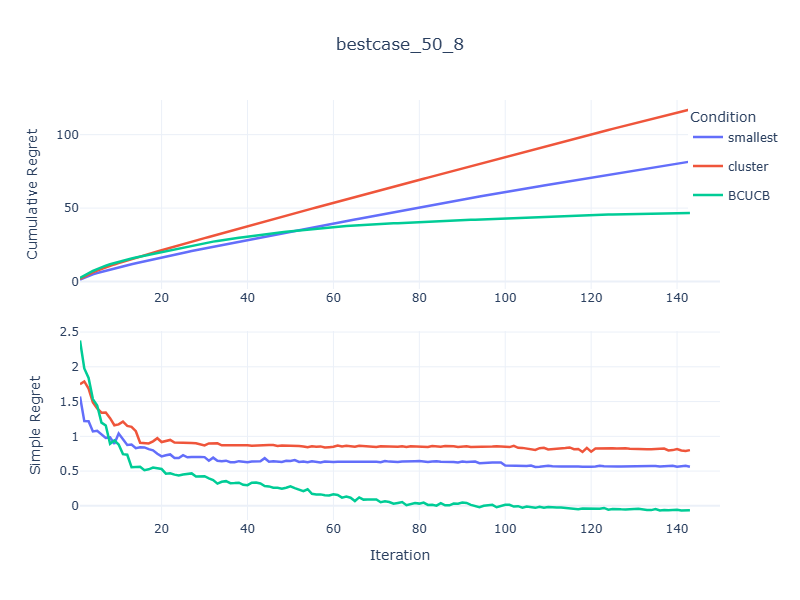
\includegraphics[width=\textwidth]{figures/best_50_8.png}
        %\caption{}
        \label{}
    \end{minipage}
    \hfill
    \begin{minipage}[t]{0.48\textwidth}
        \centering
        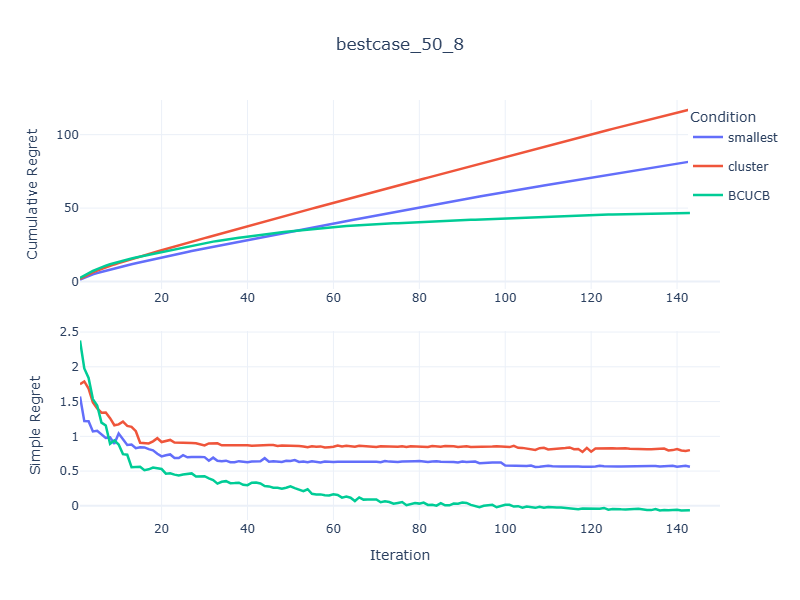
\includegraphics[width=\textwidth]{figures/best_50_16.png}
        %\caption{}
        \label{}
    \end{minipage}
    \begin{minipage}[t]{0.48\textwidth}
        \centering
        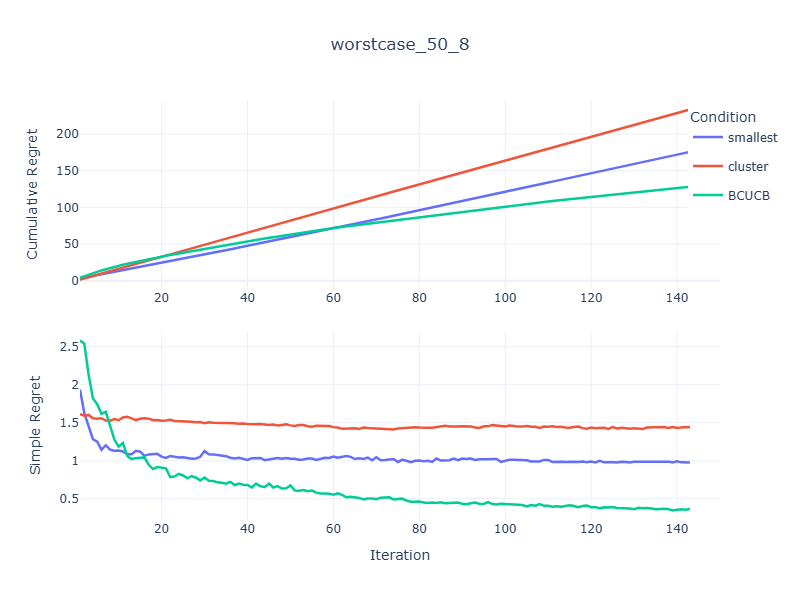
\includegraphics[width=\textwidth]{figures/worst_50_8.png}
        %\caption{}
        \label{}
    \end{minipage}
    \hfill
    \begin{minipage}[t]{0.48\textwidth}
        \centering
        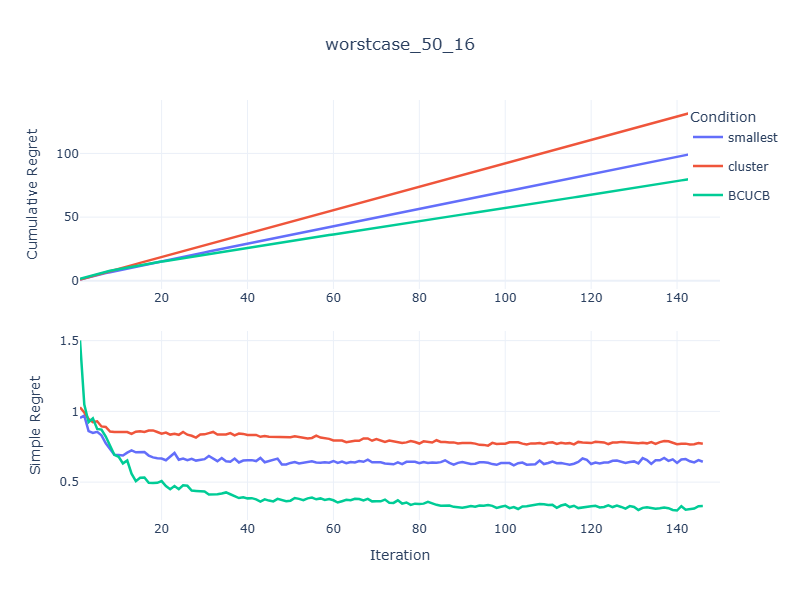
\includegraphics[width=\textwidth]{figures/worst_50_16.png}
        %\caption{}
        \label{}
    \end{minipage}
    \begin{minipage}[t]{0.48\textwidth}
        \centering
        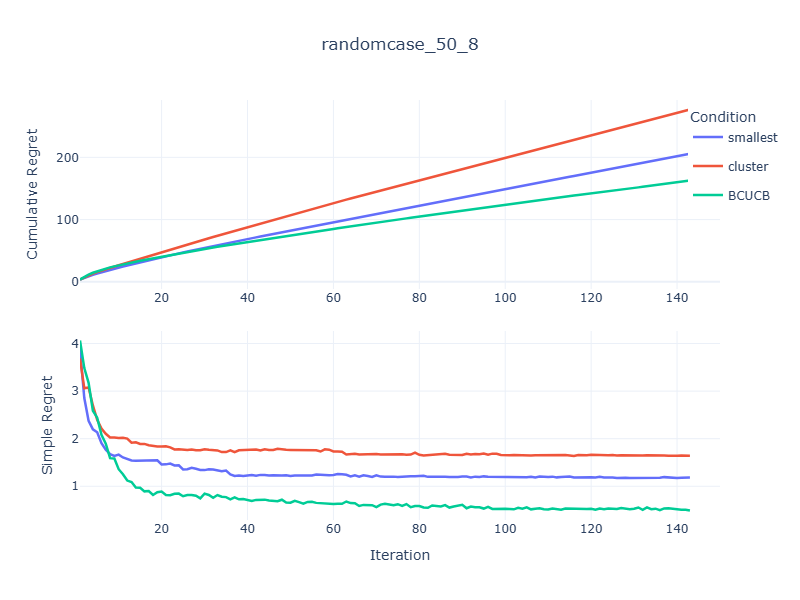
\includegraphics[width=\textwidth]{figures/random_50_8.png}
        %\caption{}
        \label{}
    \end{minipage}
    \hfill
    \begin{minipage}[t]{0.48\textwidth}
        \centering
        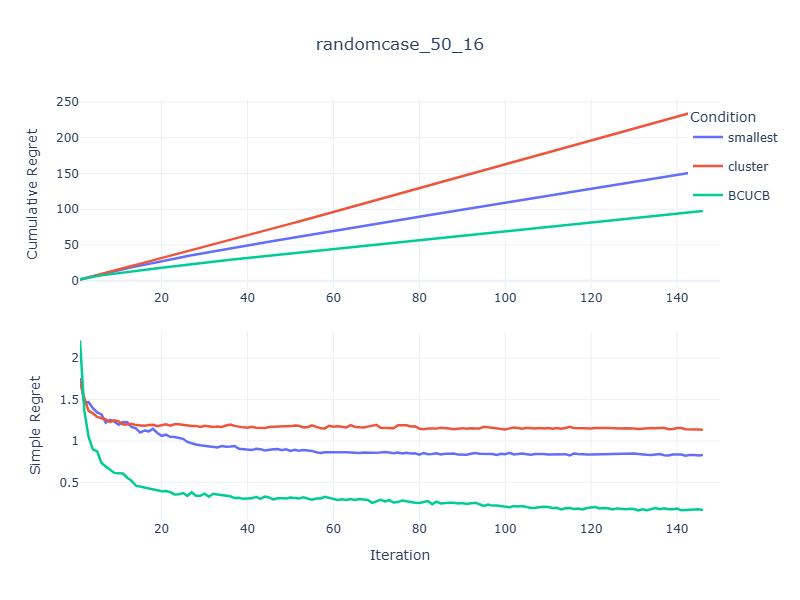
\includegraphics[width=\textwidth]{figures/random_50_16.png}
        %\caption{}
        \label{}
    \end{minipage}
\end{figure}

\begin{figure}[htbp]
    \centering
    \begin{minipage}[t]{0.48\textwidth}
        \centering
        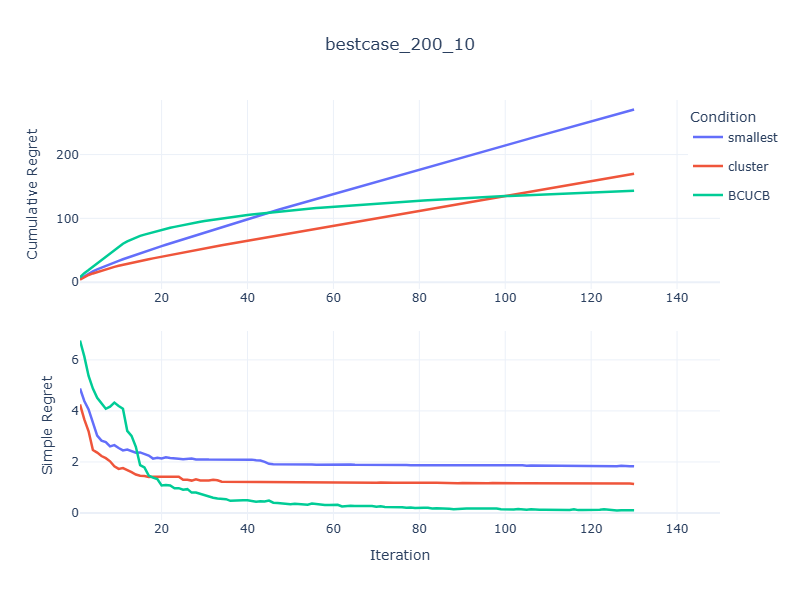
\includegraphics[width=\textwidth]{figures/best_200_10.png}
        %\caption{}
        \label{}
    \end{minipage}
    \hfill
    \begin{minipage}[t]{0.48\textwidth}
        \centering
        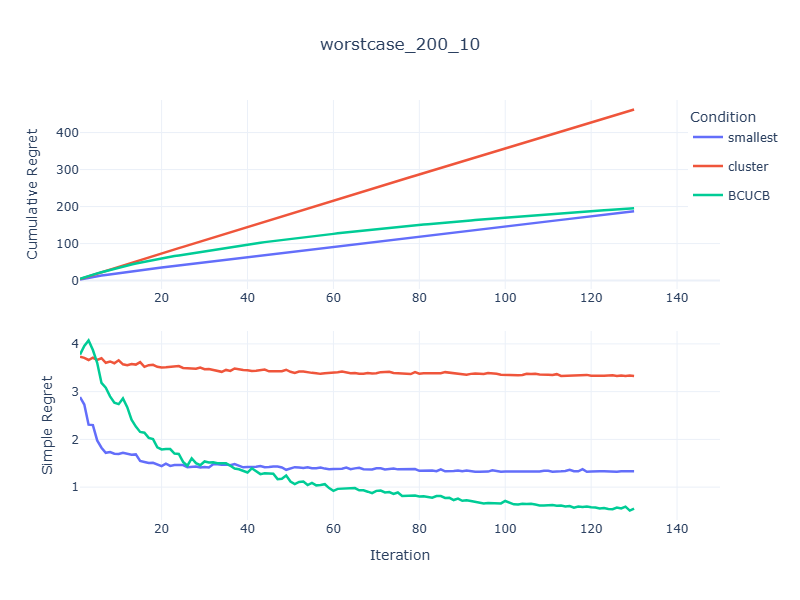
\includegraphics[width=\textwidth]{figures/worst_200_10.png}
        %\caption{}
        \label{}
    \end{minipage}
    \begin{minipage}[t]{0.48\textwidth}
        \centering
        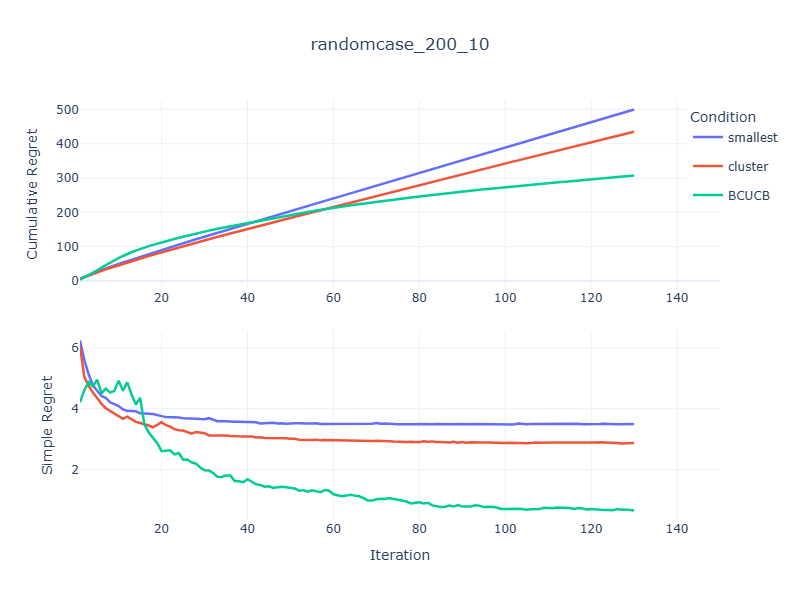
\includegraphics[width=\textwidth]{figures/random_200_10.png}
        %\caption{}
        \label{}
    \end{minipage}
\end{figure}

%--------------------------------------------------------------------------------------

\bibliographystyle{informs2014} 
\bibliography{sample} 

\ECSwitch
%%% Main head for the e-companion
\ECHead{Online Appendix}
%\begin{appendices}

\section{Proof of lemma \ref{lemma:concentration}}
\textit{Proof.} Fix $t\geq 1$ and $i\in [m]$. Conditioned on $(\mathbf{y}_1,...,\mathbf{y}_{t-1}), \{S_1,...,S_{t-1}\}$ are deterministic, and $\mu(i)\thicksim N(\mu_{t-1}(i),\sigma_{t-1}^2(i))$. Now, if $r\thicksim N(0,1)$,then: 
$$\begin{gathered}
\mathrm{Pr}\{r>c\}
\begin{aligned}
=e^{-c^2/2}(2\pi)^{-1/2}\int e^{-(r-c)^2/2-c(r-c)}dr
\end{aligned} \\
\leq e^{-c^2/2}\Pr\{r>0\}=(1/2)e^{-c^2/2}
\end{gathered}$$
for $c>0$, since $e^{-c(r-c)}\leq 1$ for $r\geq c$. Therefore, $\textnormal{Pr}\{|\mu_{t-1}(i)-\mu(i)|>\lambda_i \sigma_{t-1}(i)\}\leq e^{-\lambda_i/2}$

Assume that arm $i$ has been observed $n$ times, yielding $n$ observations. Further assume that these $n$ observations are our only observational data. Using GP modeling, we obtain:
\[
\sigma_n^2(i) = k(i,i) - \mathbf{k}_n^\top(i)(\mathbf{K}_n + \sigma^2(i)\mathbf{I}_n)^{-1}\mathbf{k}_n(i)
\]
where:
\begin{itemize}
    \item $\mathbf{k}_n(i) = [k(i,i),\dots,k(i,i)]^\top \in \mathbb{R}^n$
    \item $\mathbf{K}_n = \sigma_0^2\mathbf{1}_n\mathbf{1}_n^\top$ ($\sigma_0^2 = k(i,i)$)
\end{itemize} % itemize 已闭合

For $\mathbf{A} = \sigma^2(i)\mathbf{I}_n$, $\mathbf{u} = \sigma_0^2\mathbf{1}_n$, $\mathbf{v} = \mathbf{1}_n$, by \textbf{Sherman-Morrison} formula:
\begin{equation*}
\begin{aligned}
(\mathbf{K}_n + \sigma^2(i)\mathbf{I}_n)^{-1} &= \mathbf{A}^{-1} - \frac{\mathbf{A}^{-1}\mathbf{u}\mathbf{v}^\top\mathbf{A}^{-1}}{1 + \mathbf{v}^\top\mathbf{A}^{-1}\mathbf{u}} \\
&= \frac{1}{\sigma^2(i)}\mathbf{I}_n - \frac{\sigma_0^2/\sigma(i)^4 \cdot \mathbf{1}_n\mathbf{1}_n^\top}{1 + n\sigma_0^2/\sigma^2(i)}
\end{aligned}
\end{equation*} 

So we have:
\[
\mathbf{k}_n^\top(i)(\mathbf{K}_n + \sigma^2(i)\mathbf{I}_n)^{-1}\mathbf{k}_n(i) = \frac{\sigma_0^4n}{\sigma^2(i) + n\sigma_0^2}
\]

Substitute the results into the posterior variance formula:
\begin{equation*}
\begin{aligned}
\sigma_n^2(i) &= \sigma_0^2 - \frac{\sigma_0^4n}{\sigma^2(i) + n\sigma_0^2} = \frac{\sigma_0^2\sigma^2(i)}{\sigma^2(i) + n\sigma_0^2} \\
&= \frac{n\sigma_0^2}{\sigma^2(i)+n\sigma_0^2}\cdot \frac{\sigma^2(i)}{n} \leq \frac{\sigma^2(i)}{n}
\end{aligned}
\end{equation*} 
Considering that adding other observation points will not increase the uncertainty of arm $i$, so we have $\sigma_{t-1}(i) \leq \sigma_n(i) \leq \frac{\sigma(i)}{\sqrt{n}}$. Therefore:

$$\textnormal{Pr}\left\{|\mu_{t-1}(i)-\mu(i)|>\lambda_i \frac{\sigma(i)}{\sqrt{n}}\right\}\leq\textnormal{Pr}\{|\mu_{t-1}(i)-\mu(i)|>\lambda_i \sigma_{t-1}(i)\}\leq e^{-\lambda_i/2}$$
Denote $\epsilon_i = \lambda_i \frac{\sigma(i)}{\sqrt{n}}$, then we have $\textnormal{Pr}[|\mu_{t-1}(i)-\mu(i)|\geq \epsilon_i]\leq \exp(-\frac{n\epsilon_i^2}{2\sigma^2(i)})$  \hfill $\blacksquare$

\section{Proof of lemma \ref{lemma:lipschitz}}
\textit{Proof.} For any super arm $S = \{i_1,...,i_n\}$, denote the corresponding mean vectors in distributions $P_1$ and $P_2$ as $\boldsymbol{\mu}_{1,S} = [\mu_1(i_1),...,\mu_1(i_n)]^T$, $\boldsymbol{\mu}_{2,S} = [\mu_1(i_2),...,\mu_2(i_n)]^T$. Note that $P_1$ and $P_2$ are both multivariate normal distributions, and have same covariance matrices $\Sigma_S$.

Now, let $\mathbf{z} = [z_1,...,z_n]^T \sim N(0,\Sigma_S)$. We have:
$$
R_{P_1}(S) = \idotsint_\mathbf{z} \min \{\mu_1(i_1)+z_1,\mu_1(i_2)+z_2, \dots ,\mu_1(i_n)+z_n\} \,dz_1 \dots dz_k
$$
$$
R_{P_2}(S) = \idotsint_\mathbf{z} \min \{\mu_2(i_1)+z_1,\mu_2(i_2)+z_2, \dots ,\mu_2(i_n)+z_n\} \,dz_1 \dots dz_k
$$

Denote $f(\boldsymbol{\mu}_{1,S}+\mathbf{z}) = \min \{\mu_1(i_1)+z_1,\mu_1(i_2)+z_2, \dots ,\mu_1(i_n)+z_n\}$ and $f(\boldsymbol{\mu}_{2,S}+\mathbf{z}) = \min \{\mu_2(i_1)+z_1,\mu_2(i_2)+z_2, \dots ,\mu_2(i_n)+z_n\}$. We want to show that $f(\mu_{1,S}+\mathbf{z})-f(\mu_{2,S}+\mathbf{z})\leq \Gamma_S$.

If there exists $i,j\in S=\{i_1,...,i_n\}$ s.t. $\mu_1(i)+z_i = f(\mu_{1,S}+\mathbf{z})$, $\mu_2(j)+z_j = f(\mu_{2,S}+\mathbf{z})$, $f(\mu_{1,S}+\mathbf{z})-f(\mu_{2,S}+\mathbf{z})>\Gamma_S$. Since $\mu_1(i)+z_i = f(\mu_{1,S}+\mathbf{z}) = \min \{\mu_1(i_1)+z_1,\mu_1(i_2)+z_2, \dots ,\mu_1(i_n)+z_n\}$, we have: $\mu_1(j)+z_j> \mu_1(i)+z_i$.

Thus $\mu_1(j)-\mu_2(j) = \mu_1(j)+z_j-(\mu_2(j)+z_j)>\mu_1(i)+z_i-(\mu_2(j)+z_j)>\Gamma_S$, which is contradict with $\boldsymbol{\mu}_1 \geq \boldsymbol{\mu}_2$.

Therefore

$$
\begin{aligned}
R_{P_1}(S)-R_{P_2}(S) &= \idotsint_\mathbf{z} f(\boldsymbol{\mu}_{1,S}+\mathbf{z})-f(\boldsymbol{\mu}_{2,S}+\mathbf{z}) \,dz_1 \dots dz_k\\
&\leq \idotsint_\mathbf{z} \Gamma_S \,dz_1 \dots dz_k = \Gamma_S 
\end{aligned}
$$
\hfill $\blacksquare$

\section{Proof of lemma \ref{lemma:decomposition}}
\textit{Proof.} 
We bound the $\alpha$-approximation regret as:

\begin{equation}
    \label{eq:0}
	\begin{aligned}
		  \text{Reg}_{P,\alpha}(T) &= \sum_{t=1}^{T}\mathbb{E}\big[\alpha R_P(S^*) - R_P(S_t)\big]\\
		  &\leq \sum_{t=1}^{T}\mathbb{E}[\Delta_{S_t}]\\
		  &=\mathbb{E}[\sum_{t=1}^{m}\Delta_{S_t}]+\mathbb{E}[\sum_{t=m+1}^{T}\mathbb{I}\{\varepsilon_t\}\Delta_{S_t}]\\
		  &+\mathbb{E}[\sum_{t=m+1}^{T}\mathbb{I}\{\lnot \varepsilon_t\}\Delta_{S_t}]
	\end{aligned}
\end{equation}

(a) the first term 

Recall that $y_{\text{max}}$ is the maximum score a pilot could achieve on any module. The first term can be trivially bounded as:
\begin{equation}
	\mathbb{E}[\sum_{t=1}^{m}\Delta_{S_t}] \leq \sum_{t=1}^{m}\alpha \cdot R_P(S^*) \leq \alpha m y_{\text{max}}
\end{equation}

(b) the second term 

By Lemma 1 we know that for any $i \in [m],t\geq m+1$, denote $\gamma_i = \sigma(i)\sqrt{\frac{6\ln(t)}{T_{i,t-1}}}$, we have:
$$
	\text{Pr}[|\hat{\mu}_{t-1}(i)-\mu(i)|\geq \gamma_i] \leq \exp(-\frac{T_{i,t-1}\gamma_i^2}{2\sigma^2(i)}) = t^{-3}
$$

Therefore
\begin{equation*}
	\begin{aligned}
		\mathbb{E}[\sum_{t=m+1}^{T}\mathbb{I}\{\varepsilon_t\}]
		% &\leq \sum_{t=m+1}^{T} \sum_{i=1}^{m} \sum_{l=1}^{t-1}\text{Pr}[|\hat{\mu}_{t-1}(i)-\mu(i)|\geq \gamma_i] \\
		&\leq \sum_{t=m+1}^{T} \sum_{i=1}^{m} \sum_{l=1}^{t-1}t^{-3} \\
		&\leq m \sum_{t=m+1}^{T}t^{-2} \\
		&\leq \frac{\pi^2}{6}m
	\end{aligned}
\end{equation*}

and then the second term in (6) can be bounded as
\begin{equation}
	\begin{aligned}
		\mathbb{E}[\sum_{t=m+1}^{T}\mathbb{I}\{\varepsilon_t\}\Delta_{S_t}]&\leq \frac{\pi^2}{6}m \cdot (\alpha \cdot R_P(S^*))\\
        &\leq \frac{\pi^2}{6}\alpha m y_{\text{max}}
 	\end{aligned}
\end{equation}

(c) the third term 

We fix $t>m$ and first asuume $\lnot \varepsilon_t$ happens. Let $\gamma_i = \sigma(i)\sqrt{\frac{6\ln t}{T_{i,t-1}}}$. For each $i \in [m]$, since $\lnot \varepsilon_t$ happens, we have:
\begin{equation} 
    \label{eq:1}
	|\hat{\mu}_{T_{i,t-1}}(i)-\mu(i)| < \gamma_i ~~~ \forall i \in [m]
\end{equation}

Recall that in round $t$, the input distribution to the oracle is $P_{ucb} = \mathcal{N}(\boldsymbol{\mu}_{ucb},\Sigma)$, where the mean vector of $P_{ucb}$ satisfies:
\begin{equation}
    \label{eq:2}
	\mu_{ucb} = \hat{\mu}(i)-\gamma_i ~~~ \forall i \in [m]
\end{equation}

From \ref{eq:1} and \ref{eq:2} we  konw that $\mu(i)>\mu_{ucb}>\mu(i)-2\gamma_i$ for all $i \in [m]$. Thus, from Lemma \ref{lemma:monotonicity} we have:
\begin{equation}
    \label{eq:3}
	R_{P_{ucb}}(S)\leq R_P(S) ~~~ \forall S \in \mathcal{F}.
\end{equation}

and from Lemma \ref{lemma:lipschitz} we have:
\begin{equation}
    \label{eq:4}
	R_{P_{ucb}}(S)\geq R_P(S)-2\Gamma_S ~~~ \forall S \in \mathcal{F}.
\end{equation}
where $\Gamma_S = \mathop{\max}\limits_{i\in S}\gamma_i$

Also, from the fact that the algorithm chooses $S_t$ in the t-th round, we have:
\begin{equation}
    \label{eq:5}
	R_{P_{ucb}}(S_t)\leq \alpha \cdot \mathop{\min}\limits_{S \in \mathcal{F}}R_{P_{ucb}}(S) \leq \alpha \cdot R_{P_{ucb}}(S^*).
\end{equation}
From \ref{eq:3}, \ref{eq:4} and \ref{eq:5} we have:
\begin{equation*}
    \begin{aligned}
	R_P(S)-2\Gamma_S &\leq R_{P_{ucb}}(S_t) \leq \alpha \cdot R_{P_{ucb}}(S^*)\\
    &\leq \alpha \cdot R_P(S^*)
    \end{aligned}
\end{equation*}
which implies:
$$
	\Delta_{S_t} \leq 2\Gamma_S
$$
Therefore, when $\lnot \varepsilon_t$ happens, we always have $\Delta_{S_t}\leq 2\mathop{\max}\limits_{i\in S_t}\gamma_i$.
This implies:
$$
	\{\lnot \varepsilon_t, \Delta_{S_t}>0\}\Longrightarrow \{0<\Delta_{S_t}\leq 2\mathop{\max}\limits_{i\in S_t}\gamma_i\}=\mathcal{H}_t.
$$

Hence, the third term in (6) can be bounded as:
\begin{equation}
    \label{eq:6}
	\begin{aligned}
		\mathbb{E}[\sum_{t=m+1}^{T}\mathbb{I}\{\lnot \varepsilon_t\}\Delta_{S_t}] &= \mathbb{E}[\sum_{t=m+1}^{T}\mathbb{I}\{\lnot \varepsilon_t. \Delta_{S_t}>0\}\Delta_{S_t}]\\
		&\leq \mathbb{E}[\sum_{t=m+1}^{T}\mathbb{I}\{\mathcal{H}_t\}\Delta_{S_t}]
	\end{aligned}
\end{equation}

Finally, by combining \ref{eq:0}, \ref{eq:1}, \ref{eq:2} and \ref{eq:6}  we have:
$$
	\text{Reg}_{P,\alpha}(T) \leq \mathbb{E}[\sum_{t=m+1}^{T}\mathbb{I}\{\mathcal{H}_t\}\Delta_{S_t}] + (\frac{\pi^2}{6}+1)\alpha m y_{\text{max}}
$$
\hfill $\blacksquare$

\section{Proof of theorem \ref{thm:regret_bound}}
According to Lemma \ref{lemma:decomposition}, now it remains to bound $\mathbb{E}[\sum_{t=m+1}^{T}\mathbb{I}\{\mathcal{H}_t\}\Delta_{S_t}]$.

Define two decreasing sequences of positive contants:
$$\begin{aligned}
1 & =\beta_0>\beta_1>\beta_2>\ldots \\
 & \alpha_1>\alpha_2>\ldots
\end{aligned}$$
such that $\lim_{k \to \infty}\alpha_k = \lim_{k \to \infty}\beta_k=0$. We choose $\{\alpha_k\}$ and $\{\beta_k\}$ as in Theorem 4 of \citep{Kveton2014TightRB}, which satisfy:

\begin{equation}\sqrt{6}\sum_{k=1}^\infty\frac{\beta_{k-1}-\beta_k}{\sqrt{\alpha_k}}\leq1\end{equation}

and

\begin{equation}\sum_{k=1}^\infty\frac{\alpha_k}{\beta_k}<267.\end{equation}

For $t \in \{m+1,...,T\}$ and $k \in \mathbb{Z}_+$, let
$$m_{k,t}=
\begin{cases}
\alpha_k\left(\frac{2\sigma K}{\Delta_{S_t}}\right)^2\cdot \ln(T) & \Delta_{S_t}>0, \\
+\infty & \Delta_{S_t}=0,
\end{cases}$$

and 
$$ A_{k,t} = \{i \in S_t|T_{i,t-1}\leq m_{k,t}\}.$$

Then we define an event:
$$\mathcal{G}_{k,t}=\{|A_{k,t}|\geq\beta_kK\},$$

which means “in the $t-th$ round, at least $\beta_{k}K$ arms in $S_{t}$ had been observed at most $m_{k,t}$ times."

\begin{lemma}
In the $t-th$ round, at least $\beta_{k}K$ arms in $S_t$ had been observed at most $m_{k,t}$ times.
\end{lemma}

\textit{Proof.} Assume that $\mathcal{H}_t$ happens and that none of $\mathcal{G}_{1,t},\mathcal{G}_{2,t},...$ happens. Then $|A_{k,t}|<\beta_{k}K$ for all $k\in \mathbb{Z}_+$.

Let $A_{0,t} = S_t$ and $\bar{A}_{k,t}=S_t\setminus A_{k,t}$ for $k\in \mathbb{Z}_+\cup \{0\}$. It is easy to see $\bar{A}_{k-1,t}\subseteq\bar{A}_{k,t}$ for all $k\in \mathbb{Z}_+$. Note that $\lim_{k \to \infty}m_{k,t}=0$. Thus there exists $N\in \mathbb{Z}_+$ such that $\bar{A}_{k,t}=S_t$ for all $k\geq N$, and then we have $S_t=\bigcup_{k=1}^\infty\left(\bar{A}_{k,t}\setminus\bar{A}_{k-1,t}\right)$. Finally, note that for all $i\in \bar{A}_{k,t}$, we have $T_{i,t-1}>m_{k,t}$. Therefore
$$\begin{aligned}
\sum_{i\in S_t}\frac{1}{\sqrt{T_{i,t-1}}} & =\sum_{k=1}^\infty\sum_{i\in\bar{A}_{k,t}\setminus\bar{A}_{k-1,t}}\frac{1}{\sqrt{T_{i,t-1}}}\leq\sum_{k=1}^\infty\sum_{i\in\bar{A}_{k,t}\setminus\bar{A}_{k-1,t}}\frac{1}{\sqrt{m_{k,t}}} \\
 & =\sum_{k=1}^\infty\frac{\left|\bar{A}_{k,t}\setminus\bar{A}_{k-1,t}\right|}{\sqrt{m_{k,t}}}=\sum_{k=1}^\infty\frac{\left|A_{k-1,t}\setminus A_{k,t}\right|}{\sqrt{m_{k,t}}}=\sum_{k=1}^\infty\frac{\left|A_{k-1,t}\right|-\left|A_{k,t}\right|}{\sqrt{m_{k,t}}} \\
 & =\frac{|S_t|}{\sqrt{m_{1,t}}}+\sum_{k=1}^\infty|A_{k,t}|\left(\frac{1}{\sqrt{m_{k+1,t}}}-\frac{1}{\sqrt{m_{k,t}}}\right) \\
 & <\frac{K}{\sqrt{m_{1,t}}}+\sum_{k=1}^\infty\beta_kK\left(\frac{1}{\sqrt{m_{k+1,t}}}-\frac{1}{\sqrt{m_{k,t}}}\right) \\
 & =\sum_{k=1}^\infty\frac{(\beta_{k-1}-\beta_k)K}{\sqrt{m_{k,t}}}.
\end{aligned}$$

Note that we asuume $\mathcal{H}_t$ happens. Denote $\sigma = \mathop{\max}\limits_{i\in S_t}\sigma(i)$, then we have: 
$$\begin{aligned}
\Delta_{S_t} & \leq 2\Gamma_S=2\mathop{\max}\limits_{i\in S_t}\sigma(i)\sqrt{\frac{6\ln(t)}{T_{i,t-1}}}\\
&\leq 2\sigma \cdot \sqrt{6\ln(T)}\cdot \mathop{\max}\limits_{i\in S_t}\frac{1}{\sqrt{T_{i,t-1}}}\\
&\leq 2\sigma \cdot \sqrt{6\ln(T)}\cdot \sum_{i\in S_t}\frac{1}{\sqrt{T_{i,t-1}}}\\
&<2\sigma \cdot \sqrt{6\ln(T)}\cdot \sum_{k=1}^\infty\frac{(\beta_{k-1}-\beta_k)K}{\sqrt{m_{k,t}}}\\
&=\sqrt{6}\sum_{k=1}^\infty\frac{\beta_{k-1}-\beta_k}{\sqrt{\alpha_k}}\cdot \Delta_{S_t}\leq\Delta_{S_t},
\end{aligned}$$

We reach a contradiction here. The proof of lemma 5 is completed.
\hfill $\blacksquare$

By Lemma 5 we have
$$\sum_{t=m+1}^T\mathbb{I} \{\mathcal{H}_t\}\Delta_{S_t}\leq\sum_{k=1}^\infty\sum_{t=m+1}^T\mathbb{I}\{\mathcal{G}_{k,t},\Delta_{S_t}>0\}\Delta_{S_t}.$$

For $i\in [m], k\in \mathbb{Z}_+, t\in \{m+1,...,T\}$, define an event $\mathcal{G}_{i,k,t}=\mathcal{G}_{k,t}\wedge\{i\in S_t,T_{i,t-1}\leq m_{k,t}\}.$

Then by the definitions of $\mathcal{G}_{k,t}$ and $\mathcal{G}_{i,k,t}$ we have
$$\mathbb{I}\{\mathcal{G}_{k,t},\Delta_{S_t}>0\}\leq\frac{1}{\beta_kK}\sum_{i\in E_\mathrm{B}}\mathbb{I}\{\mathcal{G}_{i,k,t},\Delta_{S_t}>0\}.$$

Therefore
$$\sum_{t=m+1}^T\mathbb{I}\{\mathcal{H}_t\}\Delta_{S_t}\leq\sum_{i\in E_\mathrm{B}}\sum_{k=1}^\infty\sum_{t=m+1}^T\mathbb{I}\{\mathcal{G}_{i,k,t},\Delta_{S_t}>0\}\frac{\Delta_{S_t}}{\beta_kK}.$$

For each arm $i\in E_B$, suppose $i$ is contained in $N_i$ bad super arms $S_{i,1}^\mathrm{B},S_{i,2}^\mathrm{B},\ldots,S_{i,N_i}^\mathrm{B}$. Let $\Delta_{i,l} = \Delta_{S_{i,l}^\mathrm{B}}(l\in[N_i])$. Without loss of generality, we assume $\Delta_{i,1}\geq\Delta_{i,2}\geq\ldots\geq\Delta_{i,N_i}$. Note that $\Delta_{i,N_i}=\Delta_{i,\min}$. For convenience, we also define $\Delta_{i,0}=+\infty,\mathrm{~i.e.,~}\alpha_k\left(\frac{2\sigma K}{\Delta_{i,0}}\right)^2=0$. Then we have
$$\begin{aligned}
 & \sum_{t=m+1}^T\mathbb{I}\{\mathcal{H}_t\}\Delta_{S_t} \\
 & \leq\sum_{i\in E_\mathrm{B}}\sum_{k=1}^\infty\sum_{t=m+1}^T\sum_{l=1}^{N_i}\mathbb{I}\{\mathcal{G}_{i,k,t},S_t=S_{i,l}^\mathrm{B}\}\frac{\Delta_{S_t}}{\beta_kK} \\
 & \leq\sum_{i\in E_\mathrm{B}}\sum_{k=1}^\infty\sum_{t=m+1}^T\sum_{l=1}^{N_i}\mathbb{I}\{T_{i,t-1}\leq m_{k,t},S_t=S_{i,l}^\mathrm{B}\}\frac{\Delta_{i,l}}{\beta_kK} \\
 & =\sum_{i\in E_\mathrm{B}}\sum_{k=1}^\infty\sum_{t=m+1}^T\sum_{l=1}^{N_i}\mathbb{I}\left\{T_{i,t-1}\leq\alpha_k\left(\frac{2\sigma K}{\Delta_{i,l}}\right)^2\ln T,S_t=S_{i,l}^\mathrm{B}\right\}\frac{\Delta_{i,l}}{\beta_kK} \\
 & =\sum_{i\in E_{\mathrm{B}}}\sum_{k=1}^{\infty}\sum_{t=m+1}^{T}\sum_{l=1}^{N_{i}}\sum_{j=1}^{l}\mathbb{I}\left\{\alpha_k\left(\frac{2\sigma K}{\Delta_{i,j-1}}\right)^{2}\ln T<T_{i,t-1}\leq\alpha_k\left(\frac{2\sigma K}{\Delta_{i,j}}\right)^{2}\ln T,S_{t}=S_{i,l}^{\mathrm{B}}\right\}\frac{\Delta_{i,l}}{\beta_{k}K} \\
 &\leq\sum_{i\in E_{\mathrm{B}}}\sum_{k=1}^{\infty}\sum_{t=m+1}^{T}\sum_{l=1}^{N_{i}}\sum_{j=1}^{l}\mathbb{I}\left\{\alpha_k\left(\frac{2\sigma K}{\Delta_{i,j-1}}\right)^{2}\ln T<T_{i,t-1}\leq\alpha_k\left(\frac{2\sigma K}{\Delta_{i,j}}\right)^{2}\ln T,S_{t}=S_{i,l}^{\mathrm{B}}\right\}\frac{\Delta_{i,j}}{\beta_{k}K}\\
 &\leq\sum_{i\in E_{\mathrm{B}}}\sum_{k=1}^{\infty}\sum_{t=m+1}^{T}\sum_{l=1}^{N_{i}}\sum_{j=1}^{N_{i}}\mathbb{I}\left\{\alpha_k\left(\frac{2\sigma K}{\Delta_{i,j-1}}\right)^{2}\ln T<T_{i,t-1}\leq\alpha_k\left(\frac{2\sigma K}{\Delta_{i,j}}\right)^{2}\ln T,S_{t}=S_{i,l}^{\mathrm{B}}\right\}\frac{\Delta_{i,j}}{\beta_{k}K}\\
 & \leq\sum_{i\in E_\mathrm{B}}\sum_{k=1}^\infty\sum_{t=m+1}^T\sum_{j=1}^{N_i}\mathbb{I}\left\{\alpha_k\left(\frac{2\sigma K}{\Delta_{i,j-1}}\right)^2\ln T<T_{i,t-1}\leq\alpha_k\left(\frac{2\sigma K}{\Delta_{i,j}}\right)^2\ln T\right\}\frac{\Delta_{i,j}}{\beta_kK}\\
 \end{aligned}$$
$$
 \hspace{-11em}
 \begin{aligned}
 & \leq\sum_{i\in E_{\mathrm{B}}}\sum_{k=1}^{\infty}\sum_{j=1}^{N_{i}}\left(\alpha_{k}\left(\frac{2\sigma K}{\Delta_{i,j}}\right)^{2}\ln T-\alpha_{k}\left(\frac{2\sigma K}{\Delta_{i,j-1}}\right)^{2}\ln T\right)\frac{\Delta_{i,j}}{\beta_{k}K} \\
 & =4\sigma^2K\left(\sum_{k=1}^\infty\frac{\alpha_k}{\beta_k}\right)\ln T\cdot\sum_{i\in E_{\mathrm{B}}}\sum_{j=1}^{N_i}\left(\frac{1}{\Delta_{i,j}^2}-\frac{1}{\Delta_{i,j-1}^2}\right)\Delta_{i,j} \\
 & \leq1068\sigma^2K\ln T\cdot\sum_{i\in E_{\mathrm{B}}}\sum_{j=1}^{N_i}\left(\frac{1}{\Delta_{i,j}^2}-\frac{1}{\Delta_{i,j-1}^2}\right)\Delta_{i,j},
\end{aligned}
$$
where the last inequality is due to (18).

Finally, for each $i\in E_B$ we have 
$$\begin{aligned}
\sum_{j=1}^{N_i}\left(\frac{1}{\Delta_{i,j}^2}-\frac{1}{\Delta_{i,j-1}^2}\right)\Delta_{i,j} & =\frac{1}{\Delta_{i,N_i}}+\sum_{j=1}^{N_i-1}\frac{1}{\Delta_{i,j}^2}(\Delta_{i,j}-\Delta_{i,j+1}) \\
 & \leq\frac{1}{\Delta_{i,N_i}}+\int_{\Delta_{i,N_i}}^{\Delta_{i,1}}\frac{1}{x^2}\mathrm{d}x \\
 & =\frac{2}{\Delta_{i,N_i}}-\frac{1}{\Delta_{i,1}} \\
 & <\frac{2}{\Delta_{i,\min}}.
\end{aligned}$$

It follows that 
\begin{equation}
	\begin{aligned}
	\sum_{t=m+1}^T\mathbb{I}\{\mathcal{H}_t\}\Delta_{S_t}&\leq1068\sigma^2K\ln T\cdot\sum_{i\in E_\mathrm{B}}\frac{2}{\Delta_{i,\min}}\\
	&=\sigma^2K\sum_{i\in E_\mathrm{B}}\frac{2136}{\Delta_{i,\min}}\ln T.
	\end{aligned}
\end{equation}
Combining (19) with Lemma 4, the distribution-dependent regret bound in Theorem 1 is proved.

To prove the distribution-independent bound, we decompose $\sum_{t=m+1}^T\mathbb{I}\{\mathcal{H}_t\}\Delta_{S_t}$ into two parts:
\begin{equation}\begin{aligned}
\sum_{t=m+1}^T\mathbb{I}\{\mathcal{H}_t\}\Delta_{S_t}&=\sum_{t=m+1}^T\mathbb{I}\{\mathcal{H}_t,\Delta_{S_t}\leq\epsilon\}\Delta_{S_t}\\
&+\sum_{t=m+1}^T\mathbb{I}\{\mathcal{H}_t,\Delta_{S_t}>\epsilon\}\Delta_{S_t}\\
&\leq\epsilon T+\sum_{t=m+1}^T1\{\mathcal{H}_t,\Delta_{S_t}>\epsilon\}\Delta_{S_t},
\end{aligned}\end{equation}

where $\epsilon>0$ is a constant to be determined. The second term can be bounded in the same way as in the proof of the distribution-dependent regret bound, except that we only consider the case $\Delta_{S_t}>\epsilon$. Thus we can replace (19) by
\begin{equation}
	\begin{aligned}
		&\sum_{t=m+1}^T\mathbb{I}\{\mathcal{H}_t,\Delta_{S_t}>\epsilon\}\Delta_{S_t}\\
		&\leq \sigma^2K\sum_{i\in E_\mathrm{B},\Delta_{i,\min}>\epsilon}\frac{2136}{\Delta_{i,\min}}\ln T\\
		&\leq \sigma^2Km\frac{2136}{\epsilon}\ln T.
	\end{aligned}
\end{equation}

It follows that
$$\sum_{t=m+1}^T\mathbb{I}\{\mathcal{H}_t\}\Delta_{S_t}\leq\epsilon T+\sigma^2Km\frac{2136}{\epsilon}\ln T.$$

Finally, letting $\epsilon=\sqrt{\frac{2136\sigma^2Km\ln T}{T}}$, we get 
$$\sum_{t=m+1}^T\mathbb{I}\{\mathcal{H}_t\}\Delta_{S_t}\leq2\sqrt{2136\sigma^2KmT\ln T}<93\sigma\sqrt{mKT\ln T}.$$

Combining this with Lemma 4, we conclude the proof of the distribution-independent regret bound in Theorem 1.\hfill $\blacksquare$
%\end{appendices}

\section{Proof of Theorem \ref{thm:submodular}}
\textit{Proof.} Monotone Increasing is quite obvious. Here we show that $U(\cdot)$ is submodular. i.e., for any $S \subseteq T \subseteq \mathcal{X}$ and $x \in \mathcal{X} \setminus T$:
$$
U(S \cup \{x\}) - U(S) \geq U(T \cup \{x\}) - U(T).
$$
which is equivalent to:
$$
R(S)-R(S \cup \{x\}) \geq R(T) - R(T \cup \{x\}).
$$

Let $Y_S = \min_{i \in S} Y(i,\xi)$, $Y_T = \min_{i \in T} Y(i,\xi)$, $Y_x = Y(x,\xi)$. Then $Y_T \leq Y_S$. We have:
\[
R(S) - R(S \cup \{x\}) = \mathbb{E}\left[Y_S - \min\{Y_S, Y_x\}\right],
\]
\[
R(T) - R(T \cup \{x\}) = \mathbb{E}\left[Y_T - \min\{Y_T, Y_x\}\right].
\]

Consider the function $g(y) = y - \min\{y, x\}$. For fixed $x$:
\begin{itemize}
    \item If $y \leq x$, then $g(y) = 0$;
    \item If $y > x$, then $g(y) = y - x$.
\end{itemize}
Thus, $g(y)$ is non-decreasing in $y$. Since $Y_A \geq Y_B$, we have:
\[
Y_S - \min\{Y_S, Y_x\} \geq Y_T - \min\{Y_T, Y_x\}.
\]
Taking expectation:
\[
\mathbb{E}\left[Y_S - \min\{Y_S, Y_x\}\right] \geq \mathbb{E}\left[Y_T - \min\{Y_T, Y_x\}\right],
\]
which implies:
$$
U(S \cup \{x\}) - U(S) \geq U(T \cup \{x\}) - U(T).
$$
Therefore, $U(\cdot)$ is submodular.\hfill $\blacksquare$

%%%%%%%%%%%%%%%%%
\end{document}
%%%%%%%%%%%%%%%%%



